%--AMRITA UNIVERSITY B.Tech latex template--%

\documentclass[a4paper, 12pt]{report}
\usepackage[margin=0.8in]{geometry}
\usepackage{algorithm}
\usepackage{algpseudocode}
\usepackage{bold-extra}
\usepackage{amsmath}
\usepackage{amsfonts}
\usepackage{amssymb}
\usepackage{graphicx}
\usepackage[english]{babel}
\usepackage[autostyle, english = american]{csquotes}
\MakeOuterQuote{"}
\usepackage{setspace}
\onehalfspacing
\graphicspath{{images/}}
\usepackage{amsthm}
\usepackage{array}
\usepackage{cite}
\usepackage{longtable}
\usepackage{fancyhdr}
\usepackage{titletoc}
\usepackage{booktabs}
\usepackage{subcaption}
\DeclareGraphicsExtensions{.png,.jpg,.jpeg,.pdf}
\theoremstyle{definition}
\newtheorem{Definition}{Definition}[section]

%-------------------------------------------------------------
% title page
\begin{document}
	\pagenumbering{gobble}
	\thispagestyle{empty}
	\begin{large}
		\begin{center}
			{\Large\bfseries{EXPLAINABLE DEEP LEARNING APPROACH FOR SLEEP DISORDER DETECTION AND PERSONALISED LIFESTYLE RECOMMENDATIONS}}\\
			\vspace{1.3cm}
			A PROJECT REPORT \\
			\vspace{.1cm}
			Submitted in partial fulfillment for the Degree of\\
			\vspace{.1cm}
			Bachelor of Technology in\\
			Computer Science and Engineering (Artificial Intelligence)\\
			\vspace{.1cm}
			under the School of Computing\\
			\vspace{1cm}

			\normalsize Submitted by \\
\begin{table}[h]
\centering
\begin{tabular}{lr}\hline \\
Register No & Names of Students \\ \\ \hline
\\
CB.EN.U4AIE22019 & Girish Sundararajan \\
CB.EN.U4AIE22023 & Harishankar Binu Nair \\ \\ \hline
\end{tabular}
\end{table}

\vfill
			
\includegraphics[scale=0.7]{univA.png}\\
			DEPARTMENT OF COMPUTER SCIENCE AND ENGINEERING\\
			\Large{\textbf{AMRITA VISHWA VIDYAPEETHAM}}\\
			{\large Amritapuri Campus (INDIA)}\\
			\vspace*{.3cm}
			May 2025
		\end{center}
	\end{large}

	%------------------------------------------------------------------------------------
	% bonafide certificate
	\newpage
	\begin{center}
		{\large Department of Computer Science and Engineering}\\
		\Large{\textbf{AMRITA VISHWA VIDYAPEETHAM}}\\
		{\large AMRITAPURI CAMPUS}\\
		\vspace*{2.2cm}
		
\includegraphics[scale=0.5]{univA.png}\\
		\vspace*{1.5cm}
		{\Large \textbf{BONAFIDE CERTIFICATE}}
	\end{center}
	\vspace*{.8cm}
	This is to certify that this is a bonafide record of the project presented by the students whose names are given below during Project Phase II in partial fulfilment of the requirements of the degree of Bachelor of Technology in Computer Science and Engineering (Artificial Intelligence).\\[1.0cm]

\begin{table}[h]
\centering
\begin{tabular}{lr}
Roll No & Names of Students \\ \\ \hline
\\
CB.EN.U4AIE22019 & Girish Sundararajan \\
CB.EN.U4AIE22023 & Harishankar Binu Nair \\
\end{tabular}
\end{table}

\begin{flushleft}
  Dr. Simi Surendran\\
(Project Guide)\\
Assistant Professor, Department of Computer Science and Engineering\\
Amrita Vishwa Vidyapeetham, Amritapuri\\[1cm]

  Project Coordinator\\
(Project Coordinator)\\
Department of Computer Science and Engineering\\
\end{flushleft}
\begin{flushright}
Reviewer's Name\\
(Reviewer)\\
Designation
\end{flushright}

	%------------------------------------------------------------------------------------
	% declaration page
	\newpage

	\begin{center}
	    {\large Department of Computer Science and Engineering}\\
	    \Large{\textbf{AMRITA VISHWA VIDYAPEETHAM}}\\
	    {\large AMRITAPURI CAMPUS}\\
	    \vspace*{2.2cm}
	    
\includegraphics[scale=0.5]{univA.png}\\
	    \vspace*{1.5cm}
	\end{center}
	\vspace*{.8cm}

	\begin{center}
	\textbf{\Large DECLARATION}
	\end{center}

	\vspace{0.8cm}

	We, Girish Sundararajan (CB.EN.U4AIE22019) and Harishankar Binu Nair (CB.EN.U4AIE22023), hereby declare that this project entitled ``Explainable Deep Learning Approach for Sleep Disorder Detection and Personalised Lifestyle Recommendations'' is a record of the original work done by us under the guidance of Dr.\ Simi Surendran, Dept.\ of Computer Science and Engineering, Amrita Vishwa Vidyapeetham, that this work has not formed the basis for any degree/diploma/associationship/fellowship or similar awards to any candidate in any university to the best of our knowledge.

	\vspace{1.5cm}

	\noindent
	Place : Amritapuri

	\vspace{0.5cm}

	\noindent
	Date :

	\vspace{2cm}

	\begin{flushleft}
	Signature of the student
	\hfill
	Signature of the Project Guide
	\end{flushleft}

	\newpage
	%-----------------------------------------------------------------------------
	\clearpage
	\pagenumbering{roman}
	\tableofcontents

	\chapter*{Acknowledgements}
	\addcontentsline{toc}{chapter}{Acknowledgements}
We express our sincere gratitude to Dr.\ Simi Surendran, our project guide, for her consistent guidance, constructive feedback, and encouragement throughout the duration of this project. Her expertise in machine learning and her willingness to engage with the technical challenges of this work were invaluable.

We thank the Department of Computer Science and Engineering, Amrita Vishwa Vidyapeetham, Amritapuri, for providing the academic environment and resources that made this research possible.

We are grateful to the National Sleep Research Resource (NSRR) for providing licensed access to the MESA Sleep Study dataset, and to PhysioNet for maintaining the Sleep-EDF Expanded dataset as a publicly available benchmark. This work would not have been possible without these open research resources.

We thank Kaggle for providing the GPU compute infrastructure used to train the temporal-spectral fusion model, and Groq Cloud for providing the LLM inference API used in the explainability pipeline.

Finally, we thank our families and friends for their patience and support throughout the course of this project.

	\vspace{1cm}
	\begin{flushright}
		GIRISH SUNDARARAJAN\\
		HARISHANKAR BINU NAIR
	\end{flushright}
	\listoffigures
	\addcontentsline{toc}{chapter}{List of figures}
	\listoftables
	\addcontentsline{toc}{chapter}{List of tables}
	\newpage

\chapter*{Abstract}
\addcontentsline{toc}{chapter}{Abstract}

Sleep disorders affect a substantial portion of the global population, yet current diagnostic systems fragment care across separate staging and disorder detection pipelines with limited interpretability. Existing deep learning approaches achieve high accuracy but function as black boxes, preventing clinical adoption and patient engagement. This study addresses the need for a unified explainable system supporting both clinical decision making and patient self-management.

An explainable deep learning framework was developed providing unified sleep architecture analysis and disorder risk assessment. The system combines a temporal-spectral fusion model for sleep staging with multi-label classifiers for apnea, insomnia, and restless legs syndrome detection. Explainability methods operate on two levels. For clinicians, attention rollout provides per-epoch temporal influence scores, GradCAM localises signal regions driving predictions, and Monte Carlo dropout quantifies prediction uncertainty to flag cases requiring review. For patients, risk scores present disorder probabilities as percentages, feature importance highlights key contributing factors, counterfactual explanations suggest actionable changes, and a conversational interface powered by a large language model answers questions in plain language.

The framework was evaluated on the Multi-Ethnic Study of Atherosclerosis dataset containing over two thousand polysomnography recordings and the Sleep-EDF Expanded dataset for sleep staging. Sleep staging achieved macro F1 score of 0.788 with accurate detection of wake and deep sleep stages. Disorder detection achieved F1 scores of 0.784 for apnea, 0.388 for insomnia, and 0.182 for restless legs syndrome. ElasticNet stability selection improved insomnia detection by 35.9 percent over standard regularisation by preserving complementary feature groups. The explainability pipeline successfully identified uncertain predictions requiring clinician attention and generated personalised recommendations actionable by patients. Analysis confirmed that self-reported disorder labels align with behavioural features while periodic limb movement markers provide direct physiological signatures for restless legs syndrome.

The proposed framework demonstrates that a unified explainable approach can bridge the gap between accurate automated analysis and clinical utility.

\clearpage
\pagenumbering{arabic}
\setcounter{page}{1}
\chapter{Introduction}
% Chapter 1 — Introduction

\section{Background}

Sleep disorders represent one of the most prevalent yet underdiagnosed categories of chronic health conditions globally. The World Health Organization estimates that sleep disorders affect approximately one third of the adult population, with obstructive sleep apnea (OSA) alone affecting over one billion individuals worldwide. Despite this scale, the gold-standard diagnostic tool, polysomnography (PSG), remains expensive, clinically resource-intensive, and inaccessible to most patients outside tertiary care centres. Manual PSG scoring requires trained sleep technologists to classify each 30-second epoch of continuous overnight recording into one of five sleep stages according to AASM guidelines \cite{berry2020aasm}, a process that typically consumes four to eight hours per patient recording. This bottleneck creates systematic underdiagnosis, particularly for insomnia and restless legs syndrome (RLS), which lack clear physiological signatures comparable to the apnea-hypopnea events that make OSA more tractable for automated detection.

Sleep architecture is composed of five stages: wake, N1, N2, N3, and REM. Each stage is distinguished by characteristic electroencephalogram (EEG) patterns that encode distinct neurological processes \cite{supratak2017deepsleepnet, phan2022sleeptransformer}. Wake is characterised by low-amplitude, high-frequency alpha and beta activity. N1 is a transitional stage with mixed-frequency, low-amplitude activity. N2 contains sleep spindles and K-complexes. N3 is dominated by high-amplitude delta waves associated with restorative slow-wave sleep. REM sleep exhibits low-amplitude, mixed-frequency activity similar to wakefulness and is associated with dreaming and memory consolidation.

Deep learning has transformed automated sleep analysis over the past decade. Convolutional neural networks, recurrent architectures, and transformer-based models have demonstrated staging accuracies approaching inter-rater agreement on benchmark datasets \cite{phan2022sleeptransformer, fu2023tsanet, cong2025bits}. However, two critical gaps persist. First, most automated systems are trained and evaluated for sleep staging alone, treating disorder detection as a separate downstream problem disconnected from the staging pipeline. Second, existing systems produce predictions without interpretable explanations, producing what clinicians describe as black-box decisions that cannot be audited, contested, or used to support patient-facing communication.

The three most prevalent sleep disorders addressed in this project are obstructive sleep apnea, insomnia, and restless legs syndrome. Obstructive sleep apnea is characterised by recurrent upper-airway collapse during sleep, insomnia reflects hyper-arousal and difficulty maintaining sleep, and restless legs syndrome is associated with dopaminergic dysfunction leading to uncomfortable leg sensations and periodic limb movements. Epidemiological data indicate that obstructive sleep apnea affects approximately 10 to 17 percent of adults, insomnia affects 10 to 30 percent, and restless legs syndrome affects 5 to 10 percent, imposing substantial health and economic burdens \cite{rashid2022osa, karthikeyan2023insomnet, seifollahi2023osarls}.

Figure~\ref{fig:overview_intro} illustrates the overall context of this project, contrasting traditional PSG diagnosis with the proposed AI-based automated assessment framework.

\begin{figure}[h]
    \centering
    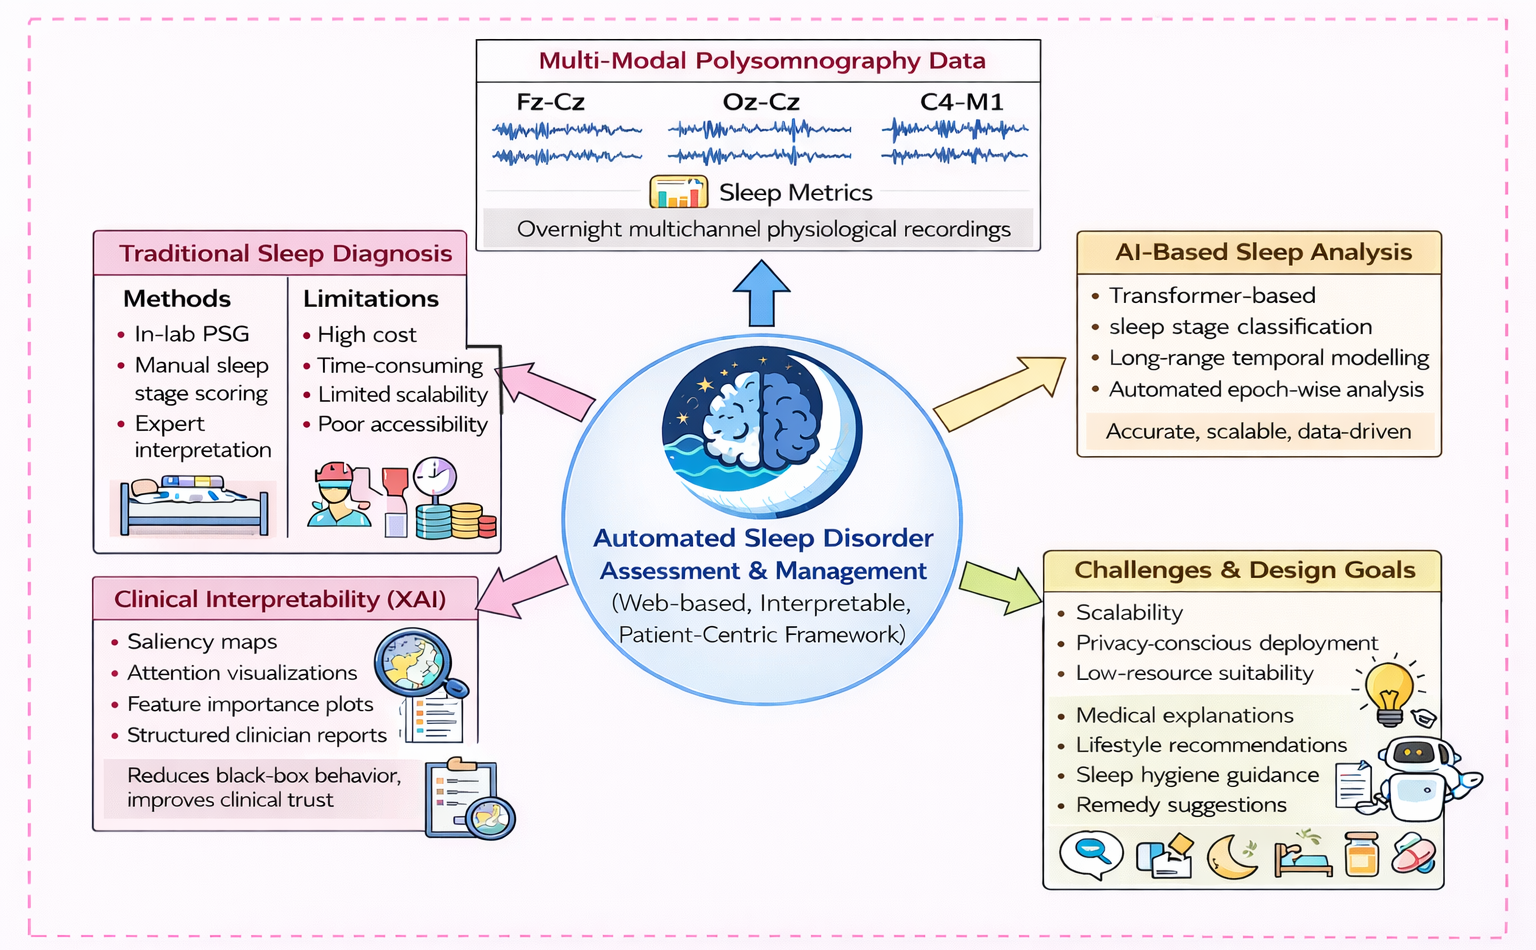
\includegraphics[width=\linewidth]{paper overview introduction figure.png}
    \caption{Overview of the automated sleep disorder assessment framework. Traditional in-lab PSG diagnosis is costly, time-consuming, and inaccessible. The proposed system replaces manual scoring with a transformer-based AI pipeline that performs sleep stage classification, disorder detection, and dual-tier explainability for both clinicians and patients.}
    \label{fig:overview_intro}
\end{figure}

\section{Problem Addressed}

Current automated PSG analysis systems share four structural limitations that this project explicitly targets.

The first limitation is single-task framing. Existing systems are optimised for staging accuracy on balanced benchmark datasets. None simultaneously addresses apnea, insomnia, and restless legs syndrome with a unified feature extraction and classification pipeline.

The second limitation is label-feature misalignment. Insomnia and RLS labels in population studies, including MESA, are self-reported, encoding diagnostic history and treatment-seeking behaviour rather than raw physiological measurements. No prior system identifies this as a root cause of poor classification performance and designs around it.

The third limitation is black-box predictions. GradCAM, attention rollout, and uncertainty quantification have been applied individually in isolation. No system integrates all three into a unified clinical review workflow with automated epoch flagging.

The fourth limitation is inaccessible patient explanation. No existing research system translates probabilistic PSG outputs into patient-readable risk scores, natural-language counterfactuals, feature importance in plain English, and an interactive conversational AI interface simultaneously.

\section{Motivation}

The primary research objective is to develop a multi-disorder sleep analysis framework that achieves clinically meaningful F1 scores for apnea, insomnia, and RLS simultaneously, not just the easiest target.

The secondary objectives are as follows. First, to design a feature selection pipeline that identifies complementary feature groups rather than standalone strong predictors, addressing the core failure of L1-only selection methods. Second, to build a temporal-spectral fusion transformer that jointly models raw EEG morphology and engineered spectral features for five-class sleep staging. Third, to produce per-epoch explainability through GradCAM event localisation, attention rollout, and Monte Carlo Dropout confidence scoring that meets clinical review standards. Fourth, to quantify prediction uncertainty per epoch to flag cases that require human review.

The research is motivated by five formal research questions. RQ1 asks whether a temporal-spectral fusion model can outperform individual-modality models for multi-disorder sleep staging. RQ2 asks whether ElasticNet bootstrap stability selection outperforms pure L1 for discovering complementary feature sets. RQ3 asks whether there is a label-feature alignment ceiling that limits PSG signal features for self-reported disorder labels. RQ4 asks whether merging PSG signal features with questionnaire features yields complementary gains, and what feature selection approach is required to realise those gains. RQ5 asks whether GradCAM combined with attention rollout can produce clinically interpretable epoch-level EEG event localisation.

\section{Scope of the Study}

This project covers the following areas. The MESA Sleep Study dataset is used for disorder classification across 2,237 subjects, accessed under a one-year research data use agreement from the National Sleep Research Resource (NSRR). The Sleep-EDF Expanded dataset is used for sleep staging across 197 overnight recordings, accessed from PhysioNet. Three disorder targets are addressed: obstructive sleep apnea, insomnia, and restless legs syndrome. Five sleep stages are classified: wake, N1, N2, N3, and REM. All model development and training is conducted in Python using PyTorch, scikit-learn, and MNE-Python on Kaggle GPU infrastructure. Large language model inference for the patient-facing explainability features uses the Groq Cloud API. Version control is managed with Git and development is conducted in Visual Studio Code.

The following areas are excluded from the current scope. Real-time inference on wearable devices is not addressed. Paediatric populations are not included. Clinical trial validation is not performed. An end-to-end EDF preprocessing backend is planned for a future phase. Cross-dataset generalisation beyond MESA and Sleep-EDF is not evaluated in this work.

The remainder of this report is organised as follows. Chapter 2 reviews existing research and tools and identifies the research gaps that motivate this work. Chapter 3 describes the proposed methodology in full, covering the datasets, preprocessing pipeline, sleep staging architecture, disorder detection pipeline, and explainability system. Chapter 4 presents experimental results, analysis, and comparative evaluation across seven experimental configurations. Chapter 5 concludes the report and outlines directions for future work. The Appendix provides key code listings from the research pipeline.

\chapter{Literature Review and Existing System}
% Chapter 2 — Literature Review / Existing System

\section{Existing System Study}

\subsection{Review of Existing Research Work}

\subsubsection{Automated Sleep Staging}

Early automated sleep staging systems relied on handcrafted feature extraction paired with traditional classifiers. Guo et al.\ \cite{guo2017hilbert} proposed a method using the Hilbert-Huang transform and sample entropy features with support vector machine classifiers, while Hassan et al.\ \cite{hassan2017decision} utilised tunable Q-factor wavelet transform with bootstrap aggregating for multi-stage classification. These approaches typically achieved accuracies ranging from 75 to 85 percent on standard benchmarks but struggled with ambiguous stages such as N1. The fundamental limitation of such methods lay in their dependence on human-engineered features, which required substantial domain expertise and often failed to capture complex physiological patterns.

The introduction of deep learning transformed the field by enabling end-to-end feature learning from raw signals. Supratak et al.\ \cite{supratak2017deepsleepnet} proposed DeepSleepNet, which combined convolutional neural networks and bidirectional long short-term memory architectures to extract time-invariant features while learning transition rules between sleep stages. Phan et al.\ \cite{phan2018deepsleepnet} extended this with SeqSleepNet, a hierarchical recurrent neural network operating on sequences of epochs rather than individual samples. While these methods improved accuracy, they functioned as black boxes, providing no mechanism for clinicians to understand model predictions.

Contemporary approaches have increasingly recognised that sleep stages exhibit distinguishing characteristics in both temporal and spectral domains. Fu et al.\ \cite{fu2023tsanet} proposed TSA-Net, a two-stream architecture extracting features simultaneously from raw EEG waveforms and spectral representations, followed by multi-head self-attention and conditional random fields for transition rule modelling. Their approach achieved 86.6 percent accuracy on Sleep-EDF-20, demonstrating that temporal-spectral fusion consistently outperformed single-modality approaches. Cong et al.\ \cite{cong2025bits} advanced this paradigm with BiTS-SleepNet, introducing cross-attention fusion that dynamically weighted temporal and spectral contributions per epoch. Their two-stage architecture combining dual-stream feature extraction with bidirectional gated recurrent units and conditional random field transition rules reached 88.5 percent accuracy on Sleep-EDF-20.

Sun and Zhao \cite{sun2025adg} proposed ADG-SleepNet, combining multi-scale dilated temporal convolutions with adaptive gating and squeeze-excitation attention, achieving 87.1 percent accuracy while maintaining computational efficiency. Huang et al.\ \cite{huang2025mhas} introduced MHASSNet, which integrated multi-scale convolution, hybrid attention mechanisms, and state space models for enhanced temporal contextual understanding. These works established hybrid convolutional-attention architectures as the dominant paradigm for high-performance sleep staging.

While accuracy improved, the interpretability challenge remained largely unaddressed until recent years. Phan et al.\ \cite{phan2022sleeptransformer} proposed SleepTransformer, the first pure transformer-based sleep staging model, which leveraged self-attention scores for interpretability at both epoch and sequence levels. Their entropy-based uncertainty quantification enabled deferral of ambiguous epochs to human experts, with experiments showing that approximately 90 percent of epochs per night could be confidently automated. Lee et al.\ \cite{lee2025sleepxvit} extended explainability to multimodal PSG inputs with SleepXViT, using layer-wise relevance propagation to generate pixel-level heatmaps aligned with AASM clinical guidelines.

Figure~\ref{fig:lit_screening} presents the systematic literature screening process used to identify the papers reviewed in this chapter.

\begin{figure}[h]
    \centering
    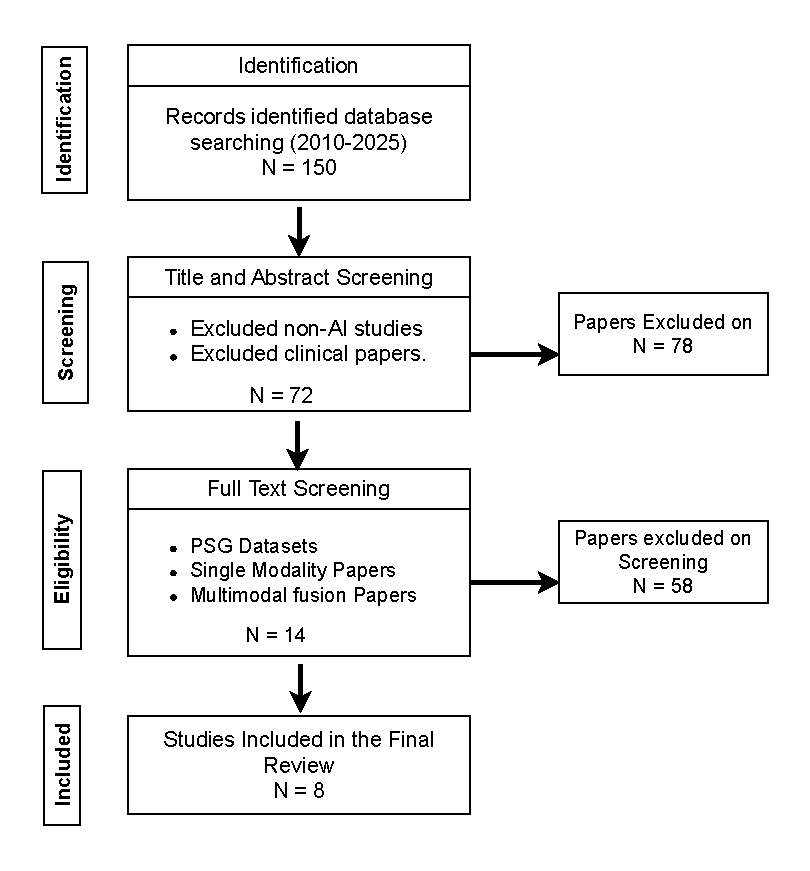
\includegraphics[width=0.85\linewidth]{literature review paper screening figure.pdf}
    \caption{Systematic literature screening process for the review of automated sleep staging and disorder detection methods. The screening covers database search, title and abstract filtering, full-text review, and final inclusion criteria.}
    \label{fig:lit_screening}
\end{figure}

\subsubsection{Sleep Disorder Detection}

Most disorder detection literature focuses exclusively on obstructive sleep apnea, using the apnea-hypopnea index computed from respiratory channels as both the detection target and the primary feature. Kim et al.\ \cite{kim2018apna} used single-channel oxygen saturation for obstructive sleep apnea screening with area under the receiver operating characteristic curve of 0.87 but without staging integration. Rashid et al.\ \cite{rashid2022osa} proposed a lightweight convolutional neural network for obstructive sleep apnea detection using single-lead ECG, achieving 94.7 percent per-recording accuracy through heart rate variability and ECG-derived respiration features.

Seifollahi et al.\ \cite{seifollahi2023osarls} addressed co-morbid obstructive sleep apnea and restless legs syndrome detection using synchrosqueezing wavelet transform of ECG and EMG signals, with multimodal fusion achieving 94.1 percent accuracy compared to 89.2 percent for ECG alone. Their work demonstrated that multi-modal fusion consistently outperformed single-modality approaches for disorder detection.

Insomnia detection presents distinct challenges due to its cognitive and behavioural components. Karthikeyan et al.\ \cite{karthikeyan2023insomnet} proposed InsomNet, utilising continuous wavelet transform of ECG signals with ResNet-LSTM architectures to achieve 93.8 percent accuracy on hospital datasets. However, they noted that questionnaire-derived insomnia labels created fundamental alignment gaps with physiological signals, limiting the achievable performance from cardiac features alone.

Few studies have attempted multi-disorder classification within unified frameworks. Islam et al.\ \cite{islam2024multishel} proposed a stacked heterogeneous ensemble learning approach combining convolutional neural networks, bidirectional LSTM, and XGBoost classifiers with SHAP explainability, achieving 96.3 percent accuracy for apnea and 94.8 percent for insomnia detection. Kumar et al.\ \cite{kumar2021lstmcnn} demonstrated LSTM-CNN hybrid architectures for four-disorder classification, attaining 88.5 percent overall accuracy using multi-modal PSG inputs. However, these ensemble and hybrid approaches incurred substantial computational costs and lacked integrated uncertainty quantification suitable for clinical workflows.

The class distribution of sleep disorders in the MESA dataset used in this work is shown in Figure~\ref{fig:disorder_dist}. The severe imbalance, with positive rates of 4.5 to 8.9 percent across the three targets, motivates the use of F1 score as the primary evaluation metric and positive class weighting in all classifiers.

\begin{figure}[h]
    \centering
    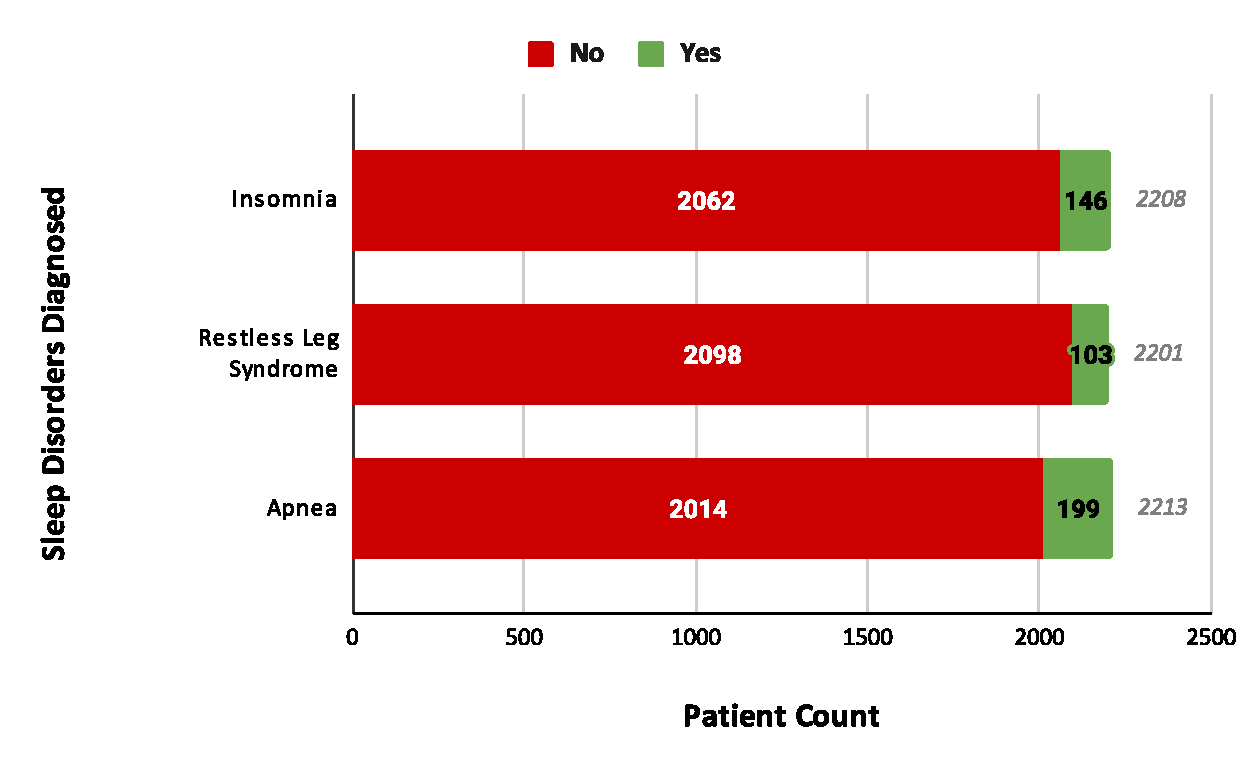
\includegraphics[width=0.75\linewidth]{sleep disorder distribution.pdf}
    \caption{Class distribution of sleep disorders in the MESA Sleep Study dataset. Positive rates are 7.6 percent for apnea, 6.3 percent for insomnia, and 4.5 percent for restless legs syndrome, reflecting the severe class imbalance that motivates F1 score as the primary evaluation metric.}
    \label{fig:disorder_dist}
\end{figure}

\subsubsection{Explainability in Sleep AI}

Selvaraju et al.\ \cite{selvaraju2017gradcam} introduced Gradient-weighted Class Activation Mapping, which computes the gradient of the class score with respect to convolutional feature maps to produce spatially localised importance maps. This method has been applied to EEG classification for epilepsy and emotion recognition but rarely for sleep staging. Attention visualisation in sleep transformers is described in SleepTransformer \cite{phan2022sleeptransformer} but is not connected to a clinical workflow with automated flagging. Monte Carlo Dropout uncertainty quantification, introduced by Gal and Ghahramani \cite{gal2016dropout}, has been applied to medical imaging but not to PSG epoch-level confidence scoring. No prior system integrates all three methods with automated flagging and a patient-facing explanation layer.

\subsection{Review of Existing Tools and Products}

The following table summarises the key commercial and research tools available for automated sleep analysis, comparing their scope, primary metric, and limitations relative to the proposed system.

\begin{table}[h]
\centering
\caption{Comparison of existing sleep analysis tools and products.}
\label{tab:tools}
\begin{tabular}{p{3.2cm}p{2.8cm}p{2.2cm}p{5cm}}
\toprule
Tool / Product & Scope & Key Metric & Limitation vs This Work \\
\midrule
ApneaLink Air (ResMed) & Apnea only & AHI, ODI & No ML, no staging, no patient UI \\
Alice NightOne (Philips) & Apnea only & AHI, SpO2 & Hardware-locked, no explainability \\
Nox T3s & Apnea only & AHI, RDI & No staging, no disorder beyond apnea \\
Somnolyzer (Siesta) & PSG staging & Stage accuracy 85\% & Proprietary, no patient-facing explanation \\
SleepSafe AI & Apnea risk & Risk category & Wearable-only, no PSG, black-box \\
This Work (Project 48) & Apnea, Insomnia, RLS + Staging & F1 = 0.784/0.388/0.182 & Unified, explainable, dual-audience outputs \\
\bottomrule
\end{tabular}
\end{table}

The table demonstrates that no existing commercial or research tool simultaneously addresses multi-disorder detection, integrates sleep staging with disorder classification, provides clinician-grade explainability, and delivers patient-accessible risk communication. This project fills all four gaps in a single unified research framework.

\section{Research Gap and Scope for Improvement}

\subsection{Gaps Addressed in This Work}

The following limitations persist in existing systems and are directly addressed by this project.

The first gap is the absence of a multi-disorder unified pipeline. No existing system addresses obstructive sleep apnea, insomnia, and restless legs syndrome simultaneously using a shared feature extraction stage and disorder-specific classifiers. Each condition is treated in isolation, preventing the system from capturing the co-morbidity patterns that are clinically prevalent.

The second gap is the uncharacterised label-feature alignment ceiling. The fundamental mismatch between self-reported disorder labels and physiological signal features has not been explicitly identified or quantified in any prior multi-disorder study. This project empirically demonstrates a 4.3-fold performance gap between questionnaire and PSG features for apnea classification, explained by the fact that self-reported labels encode diagnosis-seeking behaviour rather than raw physiology.

The third gap is the absence of integrated two-tier explainability. GradCAM epoch localisation, attention rollout, Monte Carlo Dropout confidence scoring, and automated review flagging have not been combined into a unified clinical workflow in any prior system.

The fourth gap is the lack of patient-facing AI explanation. No prior research system translates probabilistic PSG predictions into plain-English risk scores, natural-language counterfactuals, SHAP-based feature importance, and conversational AI guidance in a single integrated output.

The fifth gap is the failure of L1-only feature selection for multi-disorder detection. Pure L1 regularisation selects only standalone strong predictors and systematically discards features that are individually weak but jointly informative. This project demonstrates that ElasticNet stability selection, which combines L1 sparsity with L2 group retention, yields a 35.9 percent relative improvement in insomnia F1 score.

\subsection{Gaps Planned for Future Work}

The following gaps are identified but not addressed in the current phase. Physiological label creation from signal thresholds, specifically apnea-hypopnea index greater than 15 for apnea and periodic limb movement index greater than 15 for restless legs syndrome, would eliminate the self-reported label ceiling. Raw EMG time-series modelling for restless legs syndrome, multi-task learning with a shared encoder and three disorder-specific heads, and cross-dataset generalisation on SHHS and CHAT cohorts are all planned for the next phase.

\section{Problem Statement and Contributions}

\subsection{Problem Statement}

Existing automated PSG analysis systems are single-task, black-box, and produce outputs accessible only to specialists, creating a systematic gap between diagnostic capability and patient-accessible sleep health intelligence. No system simultaneously stages sleep, detects multiple disorders with appropriate feature selection, provides clinician-grade signal-level explainability, and delivers patient-facing personalised risk communication.

\subsection{Research Contributions}

This project makes four concrete research contributions.

The first contribution is a temporal-spectral fusion transformer architecture for five-class sleep staging. The architecture combines an Adaptive Atrous Pyramid temporal encoder with a 34-dimensional spectral encoder, achieving staging accuracy approaching state-of-the-art on the Sleep-EDF Expanded benchmark with notably strong N1 detection at 59.95 percent F1, surpassing specialised architectures including BiTS-SleepNet at 50.23 percent and SleepTransformer at 48.5 percent.

The second contribution is an ElasticNet bootstrap stability selection pipeline for multi-disorder PSG feature selection. The pipeline demonstrates that L1 plus L2 regularisation outperforms L1-only selection by 35.9 percent for insomnia through complementary feature group retention, confirming the hypothesis that insomnia requires combinations of sleep continuity metrics that are individually weak but jointly predictive.

The third contribution is the empirical characterisation of the label-feature alignment ceiling in population-based PSG studies. The project demonstrates a 4.3-fold performance ratio between questionnaire and signal features for apnea classification and explains this gap through the construct mismatch between self-reported diagnostic labels and raw physiological measurements.

The fourth contribution is the design and implementation of a two-tier explainability pipeline that serves clinicians and patients with appropriately tailored outputs. Clinicians receive GradCAM event localisation, Monte Carlo Dropout confidence scoring, and attention rollout influence scores. Patients receive accessible risk scores, SHAP-based feature importance, natural-language counterfactual explanations, and a conversational AI interface powered by the Groq Cloud LLM API. This dual-audience design is a novel contribution absent from existing automated sleep analysis research.

\chapter{Proposed Work}
% Chapter 3 — Proposed Work

\section{Proposed Work}

The proposed framework addresses the four gaps identified in Chapter 2 through a unified end-to-end pipeline for automated sleep analysis, disorder detection, and personalised explanation. The system connects directly to the research gaps as follows. The multi-disorder unified pipeline addresses the single-task framing limitation. The two-stage ElasticNet feature selection addresses the failure of L1-only methods. The two-tier explainability system addresses the black-box prediction limitation. The SomnAI patient interface addresses the inaccessible explanation limitation.

The framework integrates five modules: dual-dataset acquisition from Sleep-EDF Expanded and MESA Sleep Study; dual-stream signal preprocessing producing temporal and spectral representations for staging plus a 136-dimensional clinical feature matrix for disorder detection; a temporal-spectral fusion transformer for five-class sleep staging; an ElasticNet bootstrap stability selection pipeline feeding five machine learning classifiers for multi-disorder detection; and a two-tier explainability system serving clinicians and patients through separate output layers, with patient-facing natural language generation powered by the Groq Cloud API. The three-tier system architecture is illustrated in Figure~\ref{fig:3tier}.

\begin{figure}[h]
    \centering
    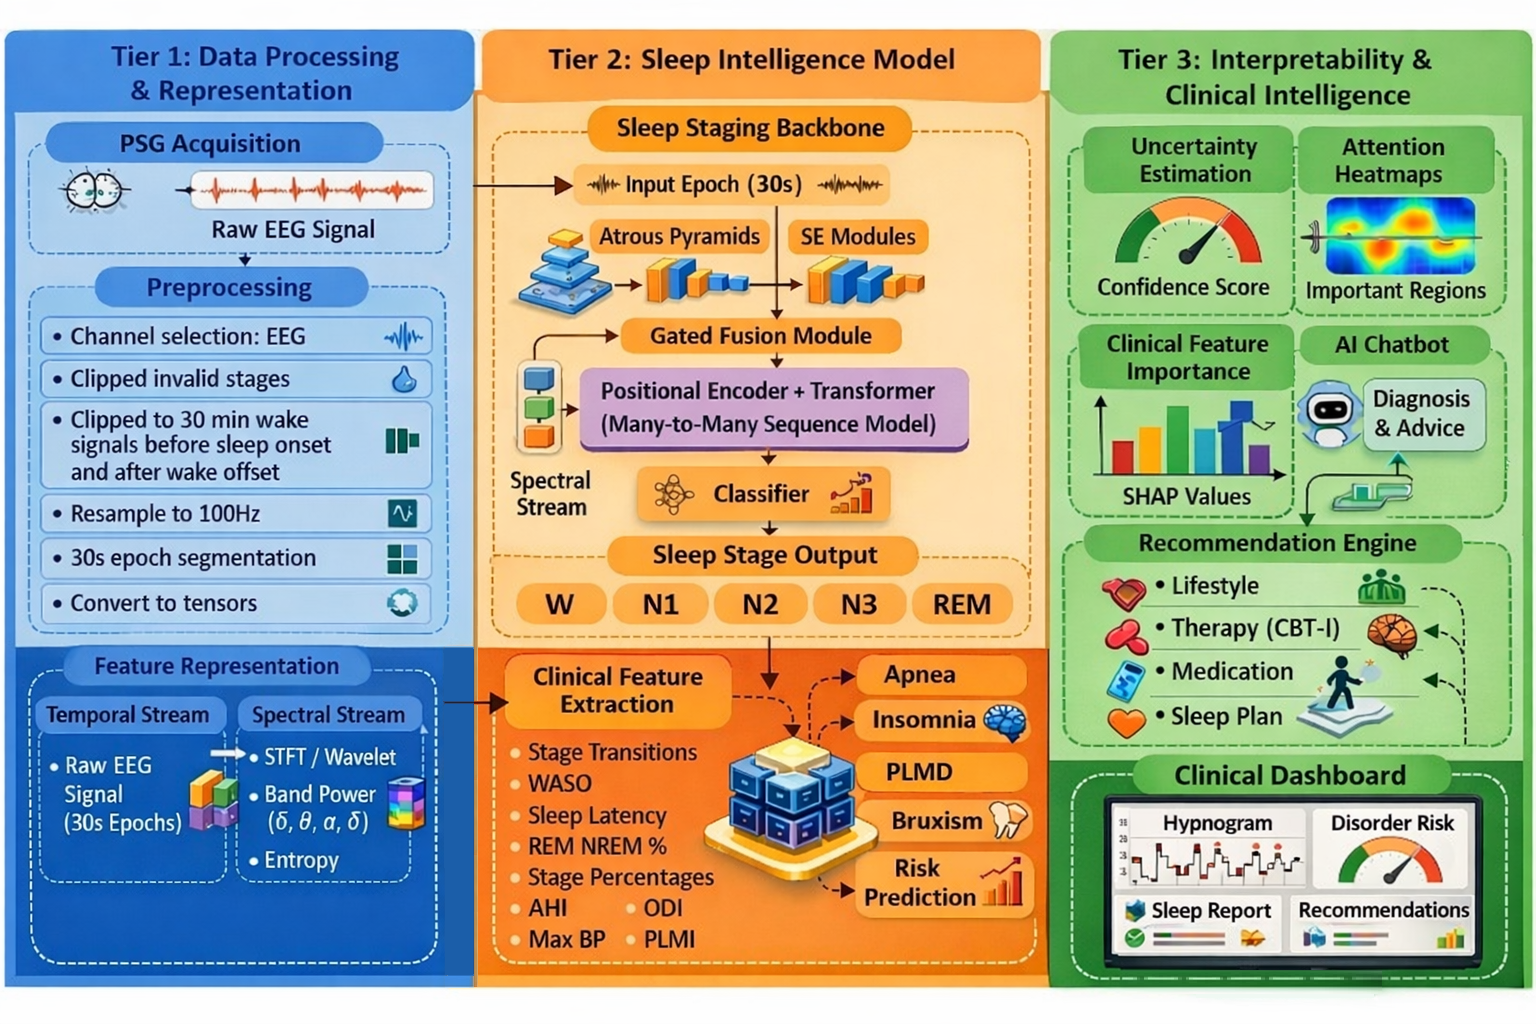
\includegraphics[width=\linewidth]{methodology 3 tier system.jpg}
    \caption{Three-tier system architecture of the proposed framework. The first tier covers data ingestion and preprocessing from multi-modal PSG recordings. The second tier performs AI-based sleep staging and disorder classification. The third tier delivers dual-audience explainability outputs: clinician-facing signal localisation and uncertainty tools, and patient-facing risk scores, feature importance, and conversational guidance via the Groq Cloud LLM API.}
    \label{fig:3tier}
\end{figure}

\subsection{Objectives of the Proposed Work}

The primary objective is to develop a multi-disorder sleep analysis framework that achieves clinically meaningful F1 scores for obstructive sleep apnea, insomnia, and restless legs syndrome simultaneously.

The secondary objectives are as follows. First, to design a feature selection pipeline that identifies complementary feature groups rather than standalone strong predictors. Second, to build a temporal-spectral fusion transformer that jointly models raw EEG morphology and engineered spectral features for five-class sleep staging. Third, to produce per-epoch explainability through GradCAM event localisation, attention rollout, and Monte Carlo Dropout confidence scoring. Fourth, to quantify prediction uncertainty per epoch to flag cases that require human review, and to generate patient-facing risk scores, feature importance, and counterfactual explanations via a Groq Cloud LLM interface.

\section{Methodology}

\subsection{Overview of the Approach}

The complete technical methodology is illustrated in Figure~\ref{fig:methodology}. The system processes two distinct input types. For sleep staging, raw EEG waveforms from the Sleep-EDF Expanded dataset are processed through a dual-stream encoder that extracts both temporal and spectral representations, which are then fused and passed through a transformer encoder for five-class epoch classification. For disorder detection, a 136-dimensional clinical feature matrix extracted from MESA PSG recordings is processed through a two-stage feature selection pipeline before being classified by an ensemble of machine learning models. The explainability pipeline operates on the outputs of both modules, generating clinician-facing attention maps and uncertainty scores alongside patient-facing risk scores and natural-language guidance.

\begin{figure}[h]
    \centering
    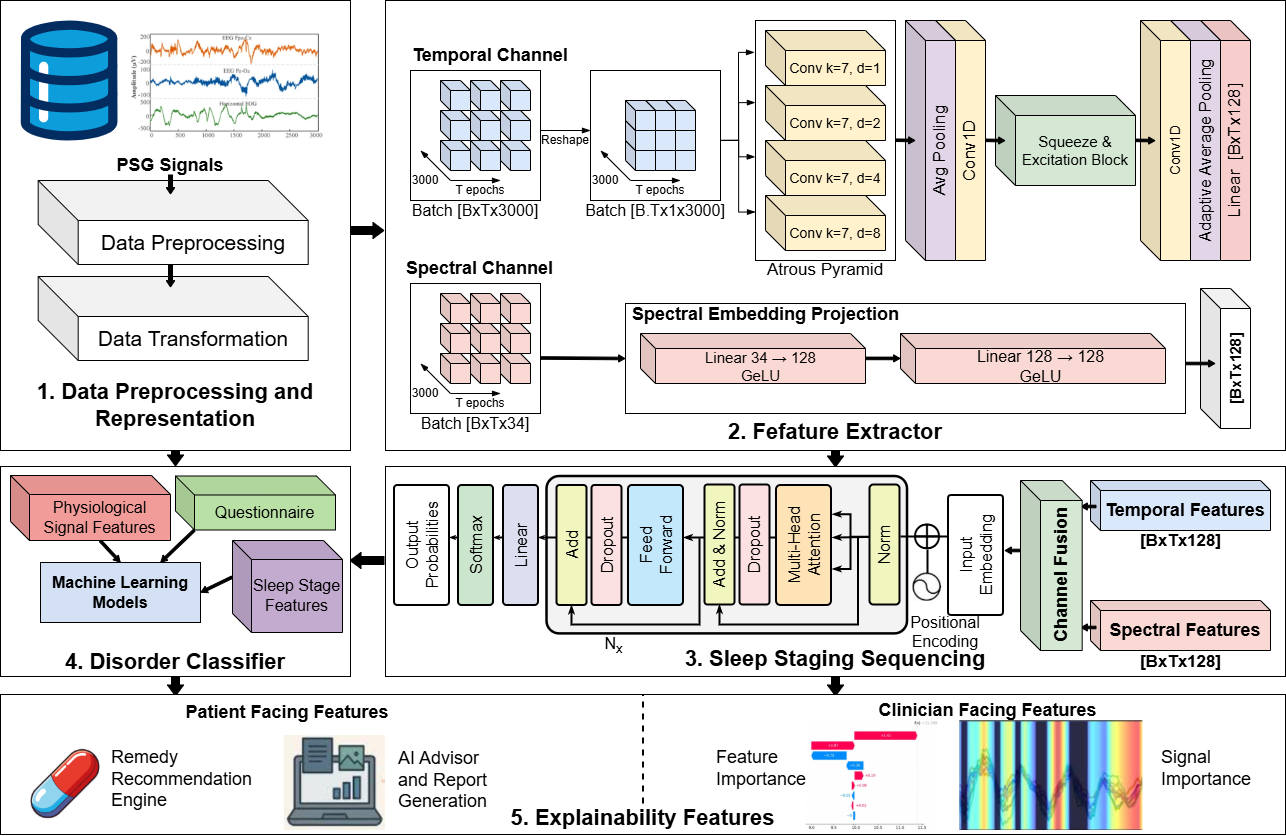
\includegraphics[width=\linewidth]{methodology_technical figure.png}
    \caption{End-to-end technical methodology of the proposed system. The pipeline covers five stages: (1) data preprocessing and dual-stream representation from PSG signals; (2) feature extraction via the Adaptive Atrous Pyramid temporal encoder and spectral embedding projection; (3) sleep staging sequencing through the transformer encoder with channel fusion; (4) disorder classification using physiological signal features, questionnaire data, and sleep stage features; and (5) explainability features split into patient-facing remedy recommendations and AI advisor, and clinician-facing feature importance and signal importance visualisations.}
    \label{fig:methodology}
\end{figure}

\subsection{Dataset Selection}

Two publicly available polysomnography datasets are used in this work.

The Sleep-EDF Expanded dataset \cite{sleepedfx}, sourced from PhysioNet \cite{physiobank}, consists of 197 whole-night PSG recordings from healthy and sleep-disturbed adult subjects spanning an age range of approximately 25 to 101 years. Data were acquired using laboratory-grade equipment with the Fpz-Cz EEG channel sampled at 100 Hz. Annotations follow the Rechtschaffen and Kales standard, segmenting recordings into 30-second epochs across five stages: wake, N1, N2, N3, and REM. This dataset is used for supervised training and validation of the sleep staging model.

The MESA Sleep Study dataset \cite{mesa2020}, accessed through the National Sleep Research Resource \cite{nsrr}, comprises over 2,200 recordings from a diverse adult cohort aged approximately 45 to 84 years. The dataset provides clinically adjudicated labels for three sleep disorders: obstructive sleep apnea, insomnia, and restless legs syndrome. These labels are derived from self-reported questionnaires, with positive class prevalence of 7.6 percent for apnea, 6.3 percent for insomnia, and 4.5 percent for restless legs syndrome. A separate PSG signal-derived feature CSV containing 2,056 rows and 136 columns was constructed from the raw MESA recordings. This dataset is used for disorder detection research.

\subsection{Algorithm and Model Design}

\subsubsection{Data Preprocessing}

The preprocessing pipeline transforms raw PSG recordings into three distinct representations.

For the sleep staging model, only the Fpz-Cz EEG channel is retained to ensure consistency across both datasets. All signals are resampled to 100 Hz to satisfy the Nyquist criterion for all clinically relevant bands up to 45 Hz. Signals are segmented into non-overlapping 30-second epochs, yielding 3,000 samples per epoch. Non-physiological labels including Movement Time and Unknown are excluded. N4 epochs are merged into N3 following current AASM conventions.

Figure~\ref{fig:eeg_stages} shows representative 30-second EEG waveforms from the Fpz-Cz channel for each sleep stage. The characteristic morphological differences are clearly visible: wake shows high-frequency, low-amplitude activity; N1 shows mixed-frequency activity; N2 shows sleep spindles and K-complexes; N3 and N4 show high-amplitude slow delta waves; and REM shows low-amplitude mixed-frequency activity resembling wake.

\begin{figure}[h]
    \centering
    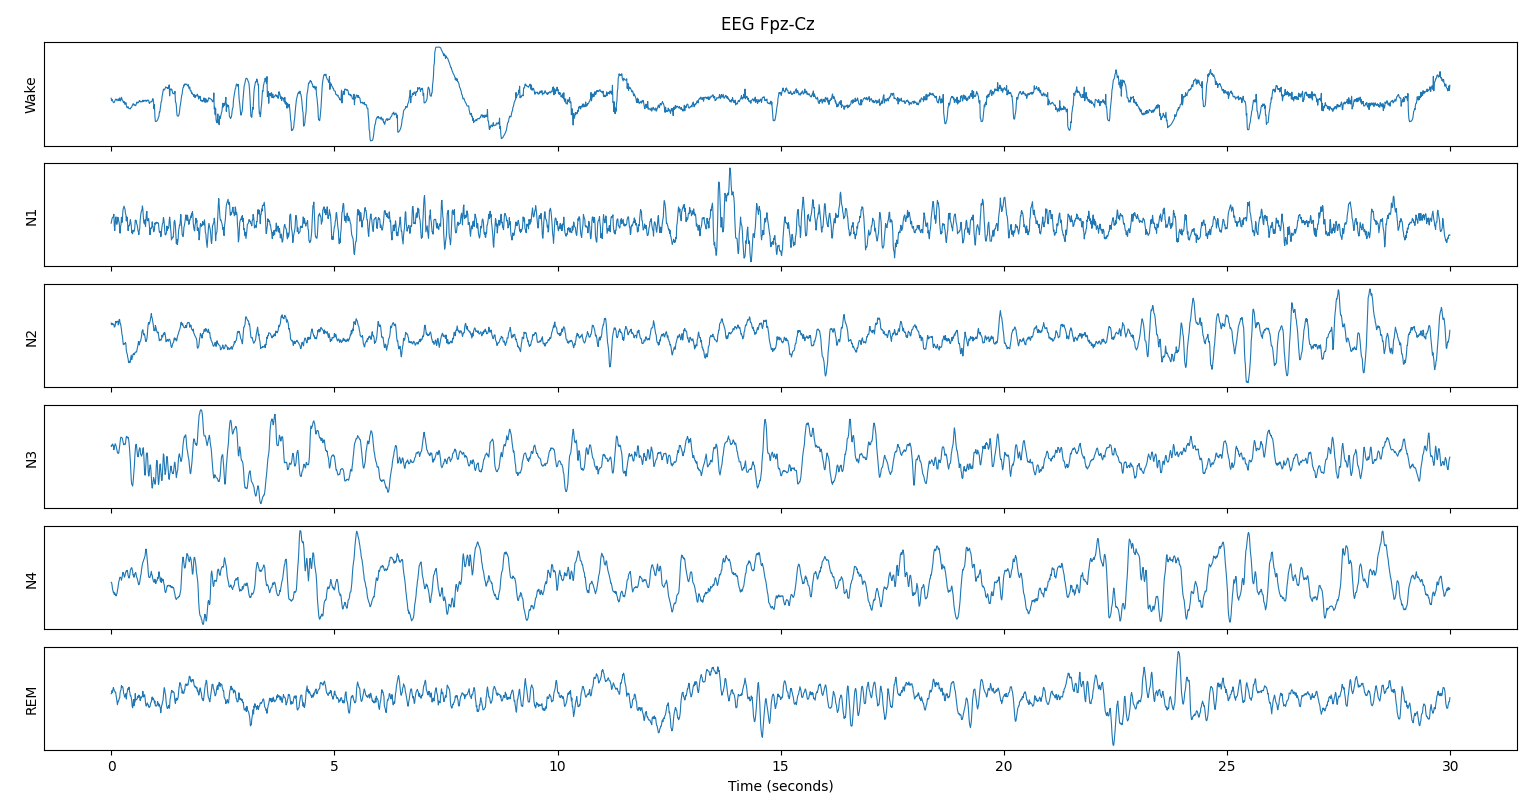
\includegraphics[width=\linewidth]{EEG Fpz-Cz vs all stages.png}
    \caption{Representative 30-second EEG Fpz-Cz waveforms for each sleep stage from the Sleep-EDF Expanded dataset. Each row shows a single epoch from wake, N1, N2, N3, N4, and REM respectively. The morphological differences between stages motivate the dual-stream temporal-spectral representation used in the proposed model.}
    \label{fig:eeg_stages}
\end{figure}

The raw Sleep-EDF Expanded dataset contains non-physiological labels and extended wake periods at recording boundaries that inflate the wake class count. Figures~\ref{fig:stage_dist_uncleaned} and~\ref{fig:stage_dist_cleaned} show the epoch distribution before and after the cleaning procedure. Before cleaning, the dataset contains 290,365 wake epochs, 25,175 N1 epochs, 88,983 N2 epochs, 12,191 N3 epochs, 7,263 N4 epochs, 34,184 REM epochs, 25,047 unscored epochs, and 211 movement epochs. After merging N4 into N3, removing non-physiological labels, and trimming boundary wake epochs, the cleaned dataset contains 44,147 wake, 25,175 N1, 88,983 N2, 19,454 N3, and 34,184 REM epochs, yielding a total of 211,943 usable epochs.

\begin{figure}[h]
    \centering
    
\includegraphics[width=\linewidth]{stages uncleaned.png}
    \caption{Sleep stage epoch distribution in the Sleep-EDF Expanded dataset before preprocessing. The raw dataset contains 290,365 wake epochs, reflecting extended pre-sleep and post-sleep recording periods, along with unscored and movement epochs that must be excluded. N4 is present as a separate class prior to AASM-compliant merging with N3.}
    \label{fig:stage_dist_uncleaned}
\end{figure}

\begin{figure}[h]
    \centering
    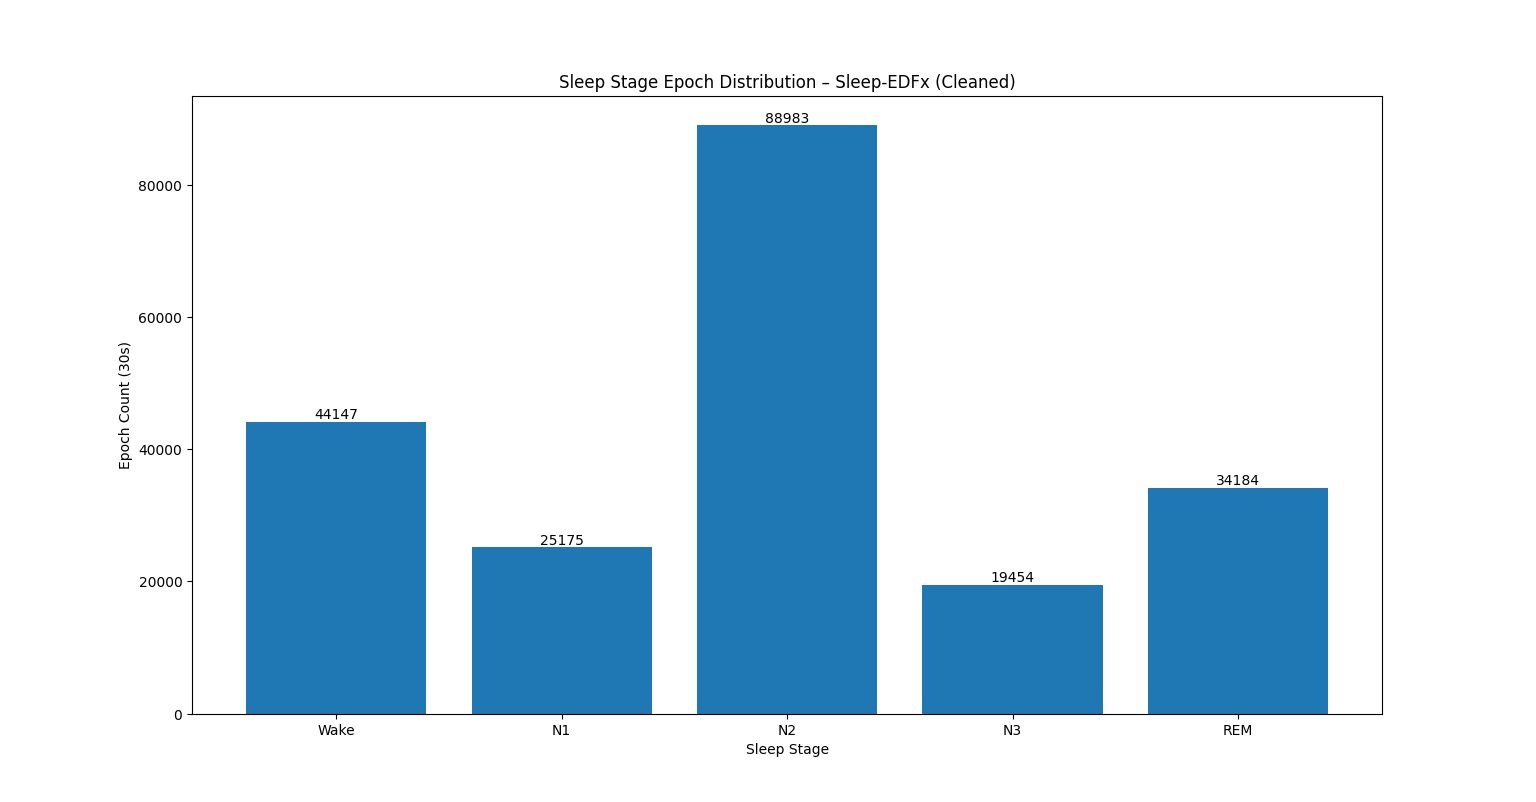
\includegraphics[width=\linewidth]{stages cleaned.png}
    \caption{Sleep stage epoch distribution after preprocessing. Non-physiological labels are removed, N4 is merged into N3, and boundary wake epochs are trimmed. The cleaned dataset contains 211,943 epochs across five classes, with N2 as the dominant stage at 88,983 epochs and N3 as the smallest at 19,454 epochs.}
    \label{fig:stage_dist_cleaned}
\end{figure}

The effect of preprocessing on the temporal structure of recordings is shown in Figures~\ref{fig:seq_uncleaned} and~\ref{fig:seq_cleaned}. Before cleaning, recordings are dominated by extended wake periods at the start and end, with sleep activity concentrated in the middle. After cleaning, the recordings show the natural ultradian sleep cycle structure with alternating NREM and REM periods across the night.

\begin{figure}[h]
    \centering
    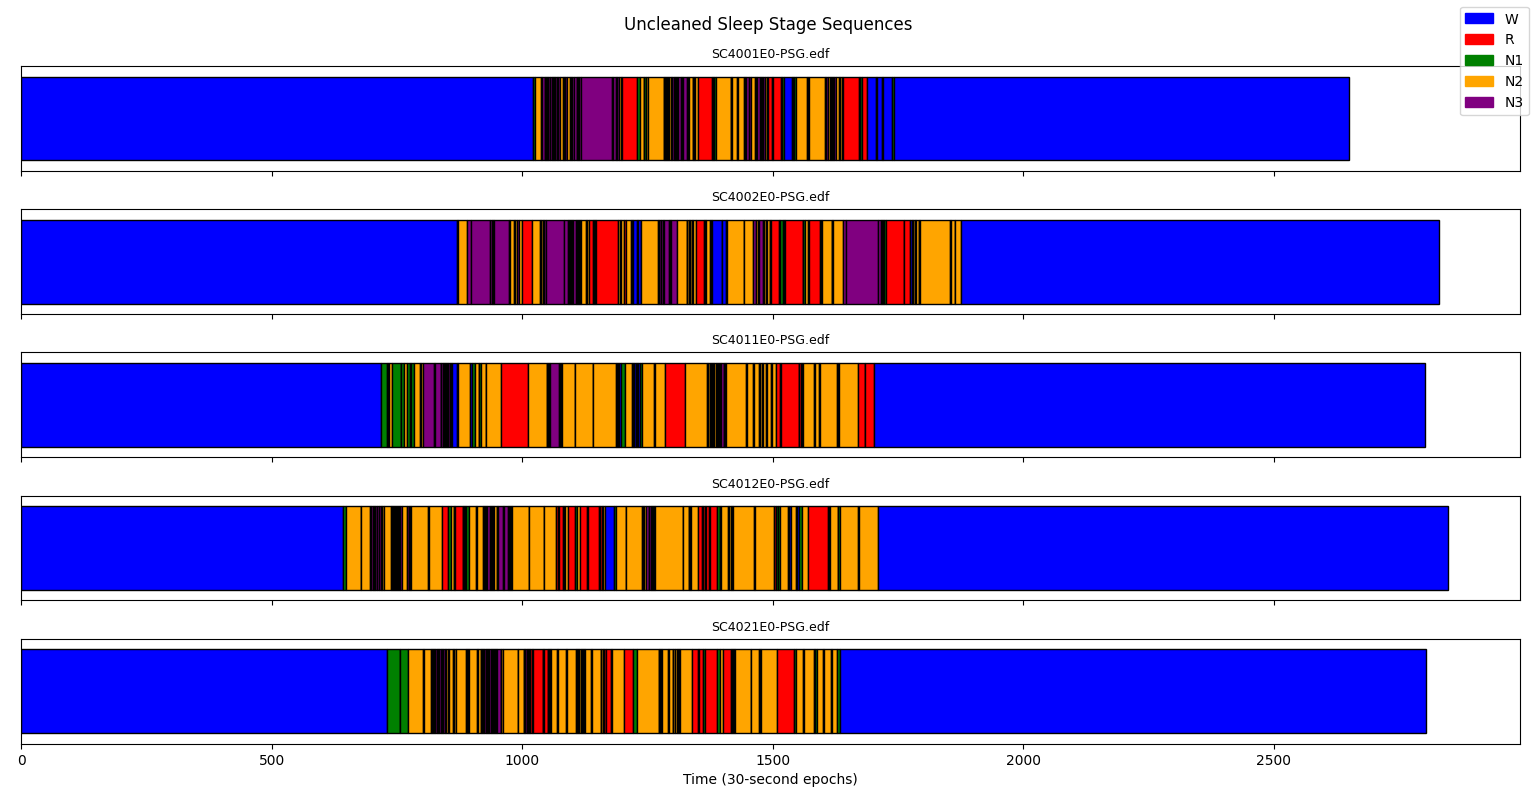
\includegraphics[width=\linewidth]{stage sequence uncleaned.png}
    \caption{Sleep stage sequences for five sample subjects before preprocessing. Each row represents one overnight recording as a colour-coded epoch timeline. The large blue (wake) regions at the start and end of each recording reflect the extended pre-sleep and post-sleep periods that are trimmed during preprocessing.}
    \label{fig:seq_uncleaned}
\end{figure}

\begin{figure}[h]
    \centering
    
\includegraphics[width=\linewidth]{stage sequence cleaned.png}
    \caption{Sleep stage sequences for the same five subjects after preprocessing. The trimmed recordings reveal the natural ultradian sleep architecture, with N3 (purple) concentrated in the first half of the night and REM (red) periods increasing in the second half, consistent with established sleep physiology.}
    \label{fig:seq_cleaned}
\end{figure}

A dual-stream representation is constructed for each epoch. The temporal stream provides the raw EEG waveform as a 3,000-dimensional vector. The spectral stream provides a 34-dimensional feature vector computed from two complementary transforms. A Discrete Wavelet Transform using the Daubechies-4 basis at decomposition level 5 extracts energy, log-energy, Shannon entropy, and variance from each decomposition level, capturing transient morphological events such as sleep spindles and K-complexes. A Short-Time Fourier Transform with a 2-second Hann window extracts relative power for the delta, theta, alpha, beta, and gamma bands, together with spectral entropy, spectral edge frequency at 95 percent, and three power ratio features. The DWT captures transient morphology that the STFT blurs, while the STFT provides stable band-power estimates that the DWT decomposes unevenly across scales. Both transforms are necessary; neither alone is sufficient.

For disorder detection, a subject-level clinical feature matrix is constructed by aggregating raw sensor signals and the output of the upstream sleep staging module. The 136-feature matrix covers seven groups: sleep architecture statistics derived from the predicted hypnogram, respiratory and apnea indices following AASM event detection criteria, oxygenation features from SpO2 analysis, cardiac and HRV features computed via Pan-Tompkins R-peak detection, periodic limb movement features from leg EMG, REM behaviour features from chin EMG, and EEG spectral power per band per stage. Preprocessing steps include median imputation for HRV zero-values arising from failed R-peak detection, exclusion of near-zero variance features, log transformation of EEG power features to normalise heavy-tailed distributions, and pruning of highly correlated feature pairs with absolute Pearson correlation exceeding 0.95.

\subsubsection{Sleep Staging Architecture}

The sleep staging module implements a temporal-spectral fusion transformer that processes both the raw EEG waveform and the pre-computed spectral feature vector for each epoch, models sequential dependencies across epochs using a transformer encoder, and classifies each epoch into one of five sleep stages.

The temporal encoder employs an Adaptive Atrous Pyramid \cite{sun2025adg} adapted for one-dimensional physiological signals. The pyramid comprises four parallel convolutional branches operating with dilation rates of 1, 2, 4, and 8, enabling simultaneous receptive fields spanning approximately 10 ms, 20 ms, 40 ms, and 80 ms at 100 Hz sampling. This multi-scale processing is motivated by the multi-temporal nature of sleep EEG: brief K-complexes and sleep spindles demand fine temporal resolution, while slow-wave oscillations require broader receptive fields. Each convolutional branch incorporates a Squeeze-and-Excitation block \cite{hu2018senet} with reduction ratio 16, which performs global average pooling across the time dimension to compute per-channel statistics, then applies a two-layer bottleneck network with sigmoid activation to produce channel-wise attention weights. Branch outputs are aggregated through a learned adaptive gating mechanism with softmax-normalised weights, and an adaptive average pooling layer reduces the temporal dimension from 3,000 samples to a 128-dimensional embedding.

The spectral encoder processes the 34-dimensional spectral feature vector through a shallow two-layer multilayer perceptron with intermediate dimension 128. Spectral features are already explicitly compressed representations of frequency content and do not require the deep hierarchical processing applied to raw waveforms.

Three fusion strategies were evaluated: concatenation, gated fusion, and bidirectional cross-attention. Ablation experiments demonstrated that simple concatenation achieves the highest staging accuracy, outperforming cross-attention fusion by 0.8 percentage points. Concatenation retains both 128-dimensional representations without suppressing any modality-specific information, whereas gating and cross-attention introduce learned compression that may discard features relevant to specific sleep stages.

The sequence model adopts a transformer encoder \cite{vaswani2017attention} with six layers, four attention heads, embedding dimension 128, feed-forward dimension 512, and sinusoidal positional encodings. The transformer models dependencies across a window of 256 epochs, effectively capturing the 90-minute ultradian sleep cycle. Global self-attention allows every epoch to attend directly to every other epoch in the window, avoiding the gradient attenuation that impairs recurrent architectures on long sequences. The output is passed to a linear classification head projecting from 128 to 5 dimensions, producing per-epoch logits over the five sleep stage classes.

The model is trained using Focal Loss \cite{lin2017focal} with gamma equal to 2.0 and per-class alpha weights to address class imbalance. The AdamW optimiser \cite{loshchilov2017adamw} is used with a ReduceLROnPlateau learning rate scheduler. Training uses a window size of 256 epochs with no overlap, and DataParallel is used for multi-GPU training on Kaggle.

Algorithm~\ref{alg:fusion} presents the pseudocode for the temporal-spectral fusion forward pass.

\begin{algorithm}[h]
\caption{Temporal-Spectral Fusion Forward Pass}\label{alg:fusion}
\begin{algorithmic}[1]
\State \textbf{Input:} $x_{\text{temp}} \in \mathbb{R}^{B \times T \times 3000}$, $x_{\text{spec}} \in \mathbb{R}^{B \times T \times 34}$
\State \textbf{Output:} logits $\in \mathbb{R}^{B \times T \times 5}$
\For{each dilation rate $d \in \{1, 2, 4, 8\}$}
    \State $h_d \gets \text{Conv1d}(x_{\text{temp}}, \text{dilation}=d)$
    \State $h_d \gets \text{SEBlock}(h_d)$
\EndFor
\State $h_{\text{temp}} \gets \text{AdaptivePool}(\text{GatedAggregate}([h_1, h_2, h_4, h_8]))$
\State $h_{\text{spec}} \gets \text{MLP}(x_{\text{spec}})$
\State $h_{\text{fused}} \gets \text{Linear}([h_{\text{temp}}; h_{\text{spec}}])$
\State $h_{\text{ctx}} \gets \text{TransformerEncoder}(h_{\text{fused}} + \text{PosEnc})$
\State \Return $\text{Linear}(h_{\text{ctx}})$
\end{algorithmic}
\end{algorithm}

\subsubsection{Sleep Disorder Detection Pipeline}

Disorder detection is formulated as multi-label binary classification for obstructive sleep apnea, insomnia, and restless legs syndrome. Independent predictions are made for each disorder per subject, recognising that the conditions frequently co-occur.

A two-stage feature selection pipeline is applied within each cross-validation fold to prevent information leakage. In the first stage, a mutual information filter with a hard threshold of 0.002 removes features with negligible marginal association with the target, reducing from 136 to approximately 80 to 100 features per disorder. In the second stage, ElasticNet bootstrap stability selection \cite{meinshausen2010stability, zou2005elasticnet} is applied over 30 resampled iterations with L1 ratio 0.5 and retention threshold 30 percent. The ElasticNet penalty balances L1 sparsity with L2 ridge regularisation, which encourages correlated features within physiological groups to remain together. This group retention property is critical for insomnia, where no single dominant feature predicts the self-reported label but combinations of sleep continuity metrics collectively encode the disorder pattern.

Five classifier architectures are evaluated. Logistic regression with ElasticNet regularisation provides a linear baseline. Random forests with 500 estimators provide non-linear feature interaction modelling. XGBoost \cite{chen2016xgboost} employs gradient-boosted trees with the ability to produce exact SHAP attributions through the TreeExplainer algorithm. Linear support vector machines provide a maximum-margin linear classifier. A multilayer perceptron implemented in PyTorch with architecture 256-128-64-1 captures non-linear feature interactions.

All models use positive class weighting equal to the ratio of negative to positive samples. Classification thresholds are tuned independently per disorder using out-of-fold probabilities from training, selecting the threshold that maximises F1 score via precision-recall curve analysis. Model evaluation uses stratified 5-fold cross-validation.

Algorithm~\ref{alg:elasticnet} presents the pseudocode for the ElasticNet bootstrap stability selection procedure.

\begin{algorithm}[h]
\caption{ElasticNet Bootstrap Stability Selection}\label{alg:elasticnet}
\begin{algorithmic}[1]
\State \textbf{Input:} $X_{\text{train}} \in \mathbb{R}^{n \times p}$, $y_{\text{train}} \in \{0,1\}^n$, $B=30$, $C=0.1$, $\lambda=0.5$, $\tau=0.30$
\State \textbf{Output:} stable feature mask $\mathbf{m} \in \{0,1\}^p$
\State $\text{counts} \gets \mathbf{0}^p$
\For{$b = 1$ to $B$}
    \State $(X_b, y_b) \gets \text{StratifiedResample}(X_{\text{train}}, y_{\text{train}})$
    \State Fit ElasticNet logistic regression with penalty $C$, L1 ratio $\lambda$
    \State $\text{counts} \mathrel{+}= \mathbf{1}[|\hat{\beta}| > 0]$
\EndFor
\State $\text{scores} \gets \text{counts} / B$
\State $\mathbf{m} \gets \mathbf{1}[\text{scores} \geq \tau]$
\State \Return $\mathbf{m}$
\end{algorithmic}
\end{algorithm}

\subsubsection{Explainability Pipeline}

The explainability pipeline produces interpretable outputs for two clinically distinct audiences.

For clinicians, attention rollout accumulates transformer attention weights across all six layers to produce per-epoch influence scores. EpochGradCAM \cite{selvaraju2017gradcam} generates within-epoch signal localisation maps by computing the gradient of the class score with respect to the feature maps of the Adaptive Atrous Pyramid projection layer. Monte Carlo Dropout uncertainty quantification \cite{gal2016dropout} provides per-epoch predictive entropy estimates by performing 30 stochastic forward passes with dropout layers forced to training mode. Predictive entropy is computed as $H = -\sum_{k} \bar{p}_k \log \bar{p}_k$. Confidence is reported using a three-tier label: ratios below 0.45 of the maximum possible entropy are reported as High confidence, ratios between 0.45 and 0.72 as Medium confidence, and ratios above 0.72 as Low confidence. Epochs are flagged for manual review when the prediction disagrees with the ground truth or when entropy exceeds the 75th percentile of the recording's entropy distribution.

For patients, predicted probabilities are converted into percentage risk scores and mapped to risk bands: low below 30 percent, moderate between 30 and 60 percent, and high above 60 percent. Feature importance is visualised using SHAP values \cite{lundberg2017shap} from the XGBoost TreeExplainer. Counterfactual explanations identify the minimum-perturbation feature change that crosses the classification threshold for each disorder, expressed in natural clinical language. A conversational AI interface uses the Groq Cloud LLM API with a system prompt that injects the patient's specific feature values and risk scores, grounds responses in the patient's actual results, and explicitly prohibits technical jargon.

\subsection{Tools and Technologies}

The research pipeline uses Python 3.10 with PyTorch 2.x for deep learning, scikit-learn 1.3 for classical machine learning, XGBoost 2.0 for gradient-boosted trees, SHAP 0.44 for feature attribution, MNE-Python 1.5 for EEG signal processing, and pandas and NumPy for data manipulation. Training is performed on Kaggle GPU instances using NVIDIA P100 and T4 GPUs. Large language model inference for the patient-facing explainability features uses the Groq Cloud API. Version control is managed with Git and development is conducted in Visual Studio Code. The MESA dataset is accessed under a one-year research data use agreement from the National Sleep Research Resource (NSRR), and the Sleep-EDF Expanded dataset is accessed from PhysioNet.

\subsection{Expected Outcomes}

The expected outcomes of this work are as follows. The temporal-spectral fusion model is expected to achieve macro F1 score above 0.78 on the Sleep-EDF Expanded benchmark, with particularly strong N1 detection due to the complementary information captured by the dual-stream architecture. The ElasticNet feature selection pipeline is expected to improve insomnia F1 by at least 30 percent relative to L1-only selection by preserving complementary sleep architecture feature groups. The explainability pipeline is expected to successfully identify uncertain predictions requiring clinician attention and generate personalised recommendations actionable by patients.

\subsection{Advantages of the Proposed Work}

The proposed system offers several advantages over existing approaches. The unified multi-disorder pipeline eliminates the need for separate systems for each condition, reducing deployment complexity and enabling the capture of co-morbidity patterns. The dual-stream temporal-spectral architecture captures complementary information from both the morphological and frequency domains of the EEG signal, outperforming single-modality approaches. The ElasticNet feature selection preserves complementary feature groups that L1-only methods discard, improving performance for disorders without single dominant predictors. The two-tier explainability system serves both clinical specialists and lay patients with appropriately tailored outputs, supporting clinical adoption and patient engagement simultaneously.

\subsection{Limitations and Assumptions}

The following limitations and assumptions apply to this work. All disorder labels are self-reported questionnaire diagnoses from the MESA dataset, encoding diagnostic history and treatment-seeking behaviour rather than objectively measured physiological severity. This label-feature alignment ceiling limits the achievable performance of models trained on PSG signal features for apnea and insomnia, regardless of model capacity. The system is trained and evaluated on two specific datasets and may not generalise to other PSG recording environments, electrode configurations, or demographic populations without retraining. The RLS detection performance remains insufficient for clinical deployment at the current stage, with the best F1 score of 0.182 indicating that aggregated periodic limb movement statistics do not adequately capture RLS pathology.

\chapter{Experimentation and Result Analysis}
% Chapter 4 — Experimentation and Result Analysis

\section{Experimental Setup}

All deep learning experiments were conducted on Kaggle GPU kernels using dual NVIDIA Tesla T4 GPUs with 30 GB combined VRAM. Classical machine learning experiments for disorder detection were run on Kaggle CPU nodes with 4 virtual CPUs and 30 GB RAM. The temporal-spectral fusion model for sleep staging was implemented in PyTorch 2.0. Disorder classification used scikit-learn 1.3, XGBoost 2.0, and PyTorch. Python 3.10 served as the primary environment, with pandas 2.0 and NumPy 1.24 for data manipulation. EEG signal processing used MNE-Python 1.5. Large language model inference for the patient-facing explainability features used the Groq Cloud API. Version control was managed with Git and development was conducted in Visual Studio Code. GPU utilisation remained between 85 and 95 percent during fusion model training.

\section{Datasets}

Two public cohorts were employed in this work.

The Sleep-EDF Expanded dataset \cite{sleepedfx} provides 197 PSG nights with Fpz-Cz EEG sampled at 100 Hz and five-class AASM sleep stage labels. The dataset was split into training and test sets using an 80/20 stratified split at the subject level with random seed 42 to prevent data leakage across subjects. After preprocessing, the cleaned dataset contains 211,943 epochs across five classes as described in Chapter 3.

The MESA Sleep Study \cite{mesa2020} provides 2,237 participants with questionnaire-derived binary disorder labels for apnea, insomnia, and restless legs syndrome, and a 136-column clinical feature matrix derived from PSG signals. The feature matrix was cleaned by replacing HRV zero-values with NaN followed by median imputation, dropping near-zero mean-HR columns, applying log transformation to spectral power features, and removing highly correlated pairs with absolute Pearson correlation exceeding 0.95.

\section{Evaluation Metrics}

Given the severe class imbalance with positive rates ranging from 4 to 9 percent across disorder targets, the primary metric is the F1 score. Classification thresholds are tuned on out-of-fold probabilities to maximise F1 per disorder rather than using the default threshold of 0.5, which would produce near-zero recall for minority classes. The secondary metric is the precision-recall area under the curve, which is invariant to threshold choice and more informative than ROC-AUC at low positive rates. ROC-AUC is reported only for historical reference and is not used for model selection, as a classifier predicting all-negative scores achieves ROC-AUC of 0.5 but F1 of 0.

\section{Experimental Design}

Seven experimental pipelines were evaluated to systematically assess the contribution of each design choice.

Experiment 1 established an RNN baseline using 9 macro sleep architecture features extracted manually from PSG recordings. Experiment 2 evaluated a manual feature set of 9 clinically chosen architecture variables including wake after sleep onset, stage percentages, total sleep time, sleep latency, and REM latency. Experiment 3 applied automated L1 feature selection using mutual information ranking followed by Lasso stability selection on the full questionnaire CSV. Experiment 4 replaced L1 with ElasticNet bootstrap stability selection to test whether the L2 component would preserve complementary feature groups. Experiment 5 evaluated PSG signal-derived features independently to assess the alignment between physiological signals and self-reported disorder labels. Experiment 6b applied a two-stage feature selection pipeline with a mutual information pre-filter at threshold 0.002 followed by ElasticNet stability selection on the merged questionnaire and PSG feature set, ensuring the features-to-samples ratio remained below 0.15. Experiment 7 trained the temporal-spectral fusion transformer on the Sleep-EDF Expanded dataset for five-class sleep staging.

Hyperparameters for the fusion model were set as follows: learning rate $10^{-3}$ with ReduceLROnPlateau decay, dropout rate 0.2, batch size 64, window size 256 epochs, and 150 training epochs. Class weights were set as $\text{pos\_weight} = n_{\text{neg}} / n_{\text{pos}}$ for all binary classifiers. Early stopping with patience of 10 epochs on validation loss was applied to the PyTorch MLP in disorder detection experiments.

\section{Results}

\subsection{Sleep Staging Ablation Study}

Table~\ref{tab:ablation} presents the results of the ablation study comparing temporal-only, spectral-only, and fusion architectures on the Sleep-EDF Expanded dataset. The temporal-only model achieves macro F1 of 0.191, with N2 detection at 0.534 but complete failure on N1, N3, and REM. The spectral-only model achieves macro F1 of 0.582 with balanced performance across all stages. All three fusion variants substantially outperform single-modality approaches, with concatenation fusion achieving the highest macro F1 of 0.788.

\begin{table}[h]
\centering
\caption{Ablation study comparing single-modality and fusion architectures. MF1 denotes macro F1 score. All values are F1 scores per class.}
\label{tab:ablation}
\begin{tabular}{lcccccc}
\toprule
Architecture & Wake & N1 & N2 & N3 & REM & MF1 \\
\midrule
Temporal Only & 0.420 & 0.000 & 0.534 & 0.000 & 0.000 & 0.191 \\
Spectral Only & 0.780 & 0.250 & 0.740 & 0.680 & 0.460 & 0.582 \\
Cross-Attention Fusion & 0.911 & 0.588 & 0.754 & 0.758 & 0.889 & 0.780 \\
Gated Fusion & 0.911 & 0.600 & 0.763 & 0.748 & 0.893 & 0.783 \\
Concatenation Fusion & 0.917 & 0.600 & 0.765 & 0.768 & 0.889 & \textbf{0.788} \\
\bottomrule
\end{tabular}
\end{table}

The normalised confusion matrices for the temporal-only and spectral-only baselines are shown in Figures~\ref{fig:cm_temporal} and~\ref{fig:cm_spectral}. The temporal-only model collapses predictions toward N3 and REM, with zero recall for N2. The spectral-only model shows a more balanced distribution but still misclassifies a substantial fraction of N2 epochs as N1.

\begin{figure}[h]
    \centering
    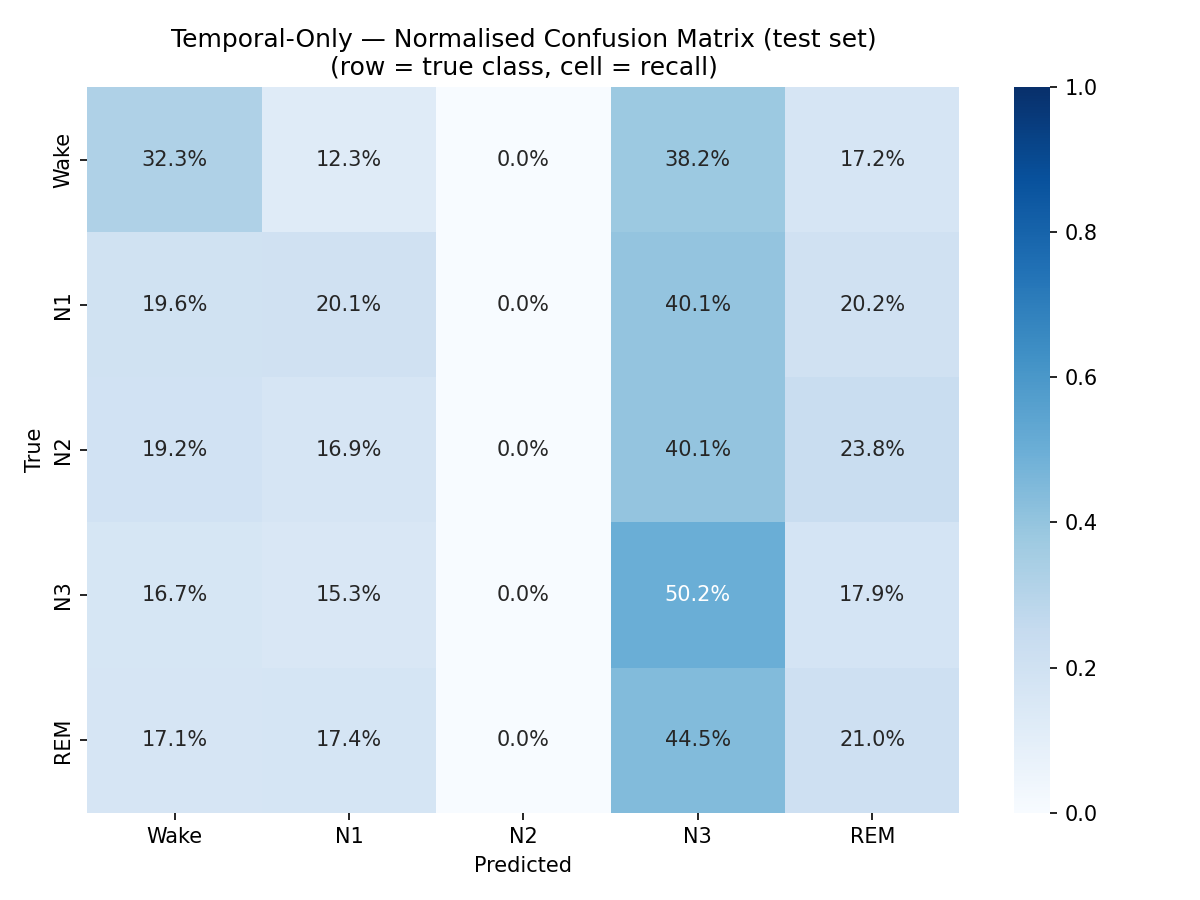
\includegraphics[width=0.65\linewidth]{confusion_matrix_temporal_only_test_normalised.png}
    \caption{Normalised confusion matrix for the temporal-only baseline model. The model fails to classify N2 epochs entirely (0\% recall), collapsing predictions toward N3 and distributing errors broadly across all classes. This confirms that raw EEG waveforms alone are insufficient for reliable five-class staging without spectral guidance.}
    \label{fig:cm_temporal}
\end{figure}

\begin{figure}[h]
    \centering
    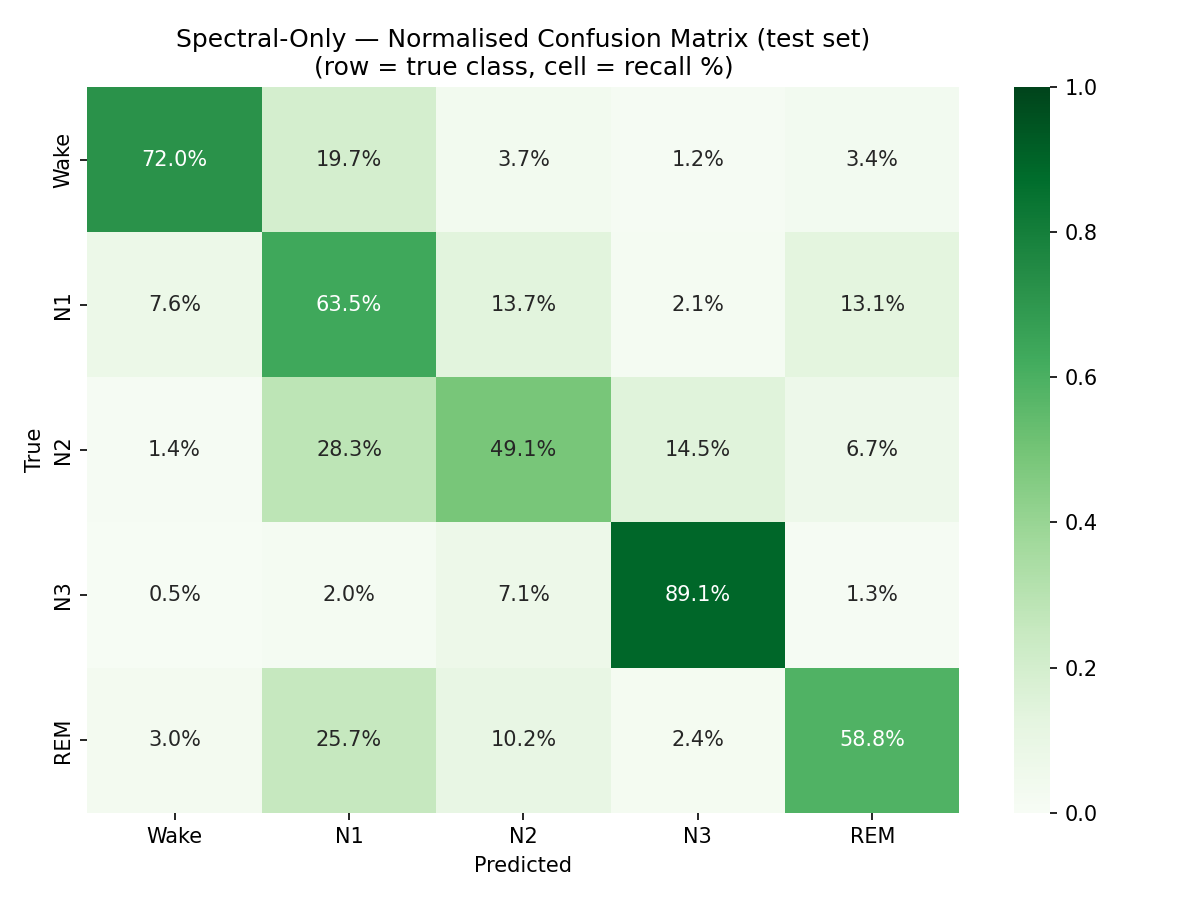
\includegraphics[width=0.65\linewidth]{confusion_matrix_spectral_only_test_normalised.png}
    \caption{Normalised confusion matrix for the spectral-only baseline model. Performance is substantially better than temporal-only, with N3 recall at 89.1\% and N1 recall at 63.5\%. However, N2 recall is only 49.1\%, with significant confusion toward N1, motivating the addition of the temporal stream to capture morphological transients.}
    \label{fig:cm_spectral}
\end{figure}

\subsection{Merged Per-Class Metrics for All Fusion Variants}

Table~\ref{tab:perclass_merged} presents the merged per-class precision, recall, and F1 scores for all three fusion variants alongside the two single-modality baselines, extracted from the classification reports. This consolidated view enables direct comparison of how each architecture handles each sleep stage.

\begin{table}[h]
\centering
\caption{Merged per-class classification metrics for all architectures. P = Precision, R = Recall, F1 = F1 score. Best F1 per class shown in bold.}
\label{tab:perclass_merged}
\begin{tabular}{llccccccccccccccc}
\toprule
& & \multicolumn{3}{c}{Wake} & \multicolumn{3}{c}{N1} & \multicolumn{3}{c}{N2} & \multicolumn{3}{c}{N3} & \multicolumn{3}{c}{REM} \\
\cmidrule(lr){3-5}\cmidrule(lr){6-8}\cmidrule(lr){9-11}\cmidrule(lr){12-14}\cmidrule(lr){15-17}
Architecture & Acc & P & R & F1 & P & R & F1 & P & R & F1 & P & R & F1 & P & R & F1 \\
\midrule
Temporal Only & -- & -- & -- & 0.42 & -- & -- & 0.00 & -- & -- & 0.53 & -- & -- & 0.00 & -- & -- & 0.00 \\
Spectral Only & -- & -- & -- & 0.78 & -- & -- & 0.25 & -- & -- & 0.74 & -- & -- & 0.68 & -- & -- & 0.46 \\
Cross-Attn & 79.1\% & 0.983 & 0.849 & 0.911 & 0.437 & 0.900 & 0.588 & 0.961 & 0.621 & 0.754 & 0.618 & 0.982 & 0.758 & 0.852 & 0.928 & 0.889 \\
Gated Fusion & 79.5\% & 0.987 & 0.847 & 0.911 & 0.448 & 0.906 & 0.600 & 0.964 & 0.631 & 0.763 & 0.604 & 0.983 & 0.748 & 0.860 & 0.928 & 0.893 \\
Concat Fusion & \textbf{79.9\%} & 0.984 & 0.858 & \textbf{0.917} & 0.447 & 0.911 & \textbf{0.600} & 0.958 & 0.637 & \textbf{0.765} & 0.634 & 0.973 & \textbf{0.768} & 0.862 & 0.918 & \textbf{0.889} \\
\bottomrule
\end{tabular}
\end{table}

\subsection{Confusion Matrices for Fusion Variants}

Figures~\ref{fig:cm_concat}, \ref{fig:cm_gated}, and~\ref{fig:cm_crossattn} show the count and normalised confusion matrices for the three fusion variants. All three variants show strong diagonal classification for wake, N3, and REM. The concatenation fusion achieves the best N3 recall at 97.32 percent and the best overall accuracy at 79.91 percent.

\begin{figure}[h]
    \centering
    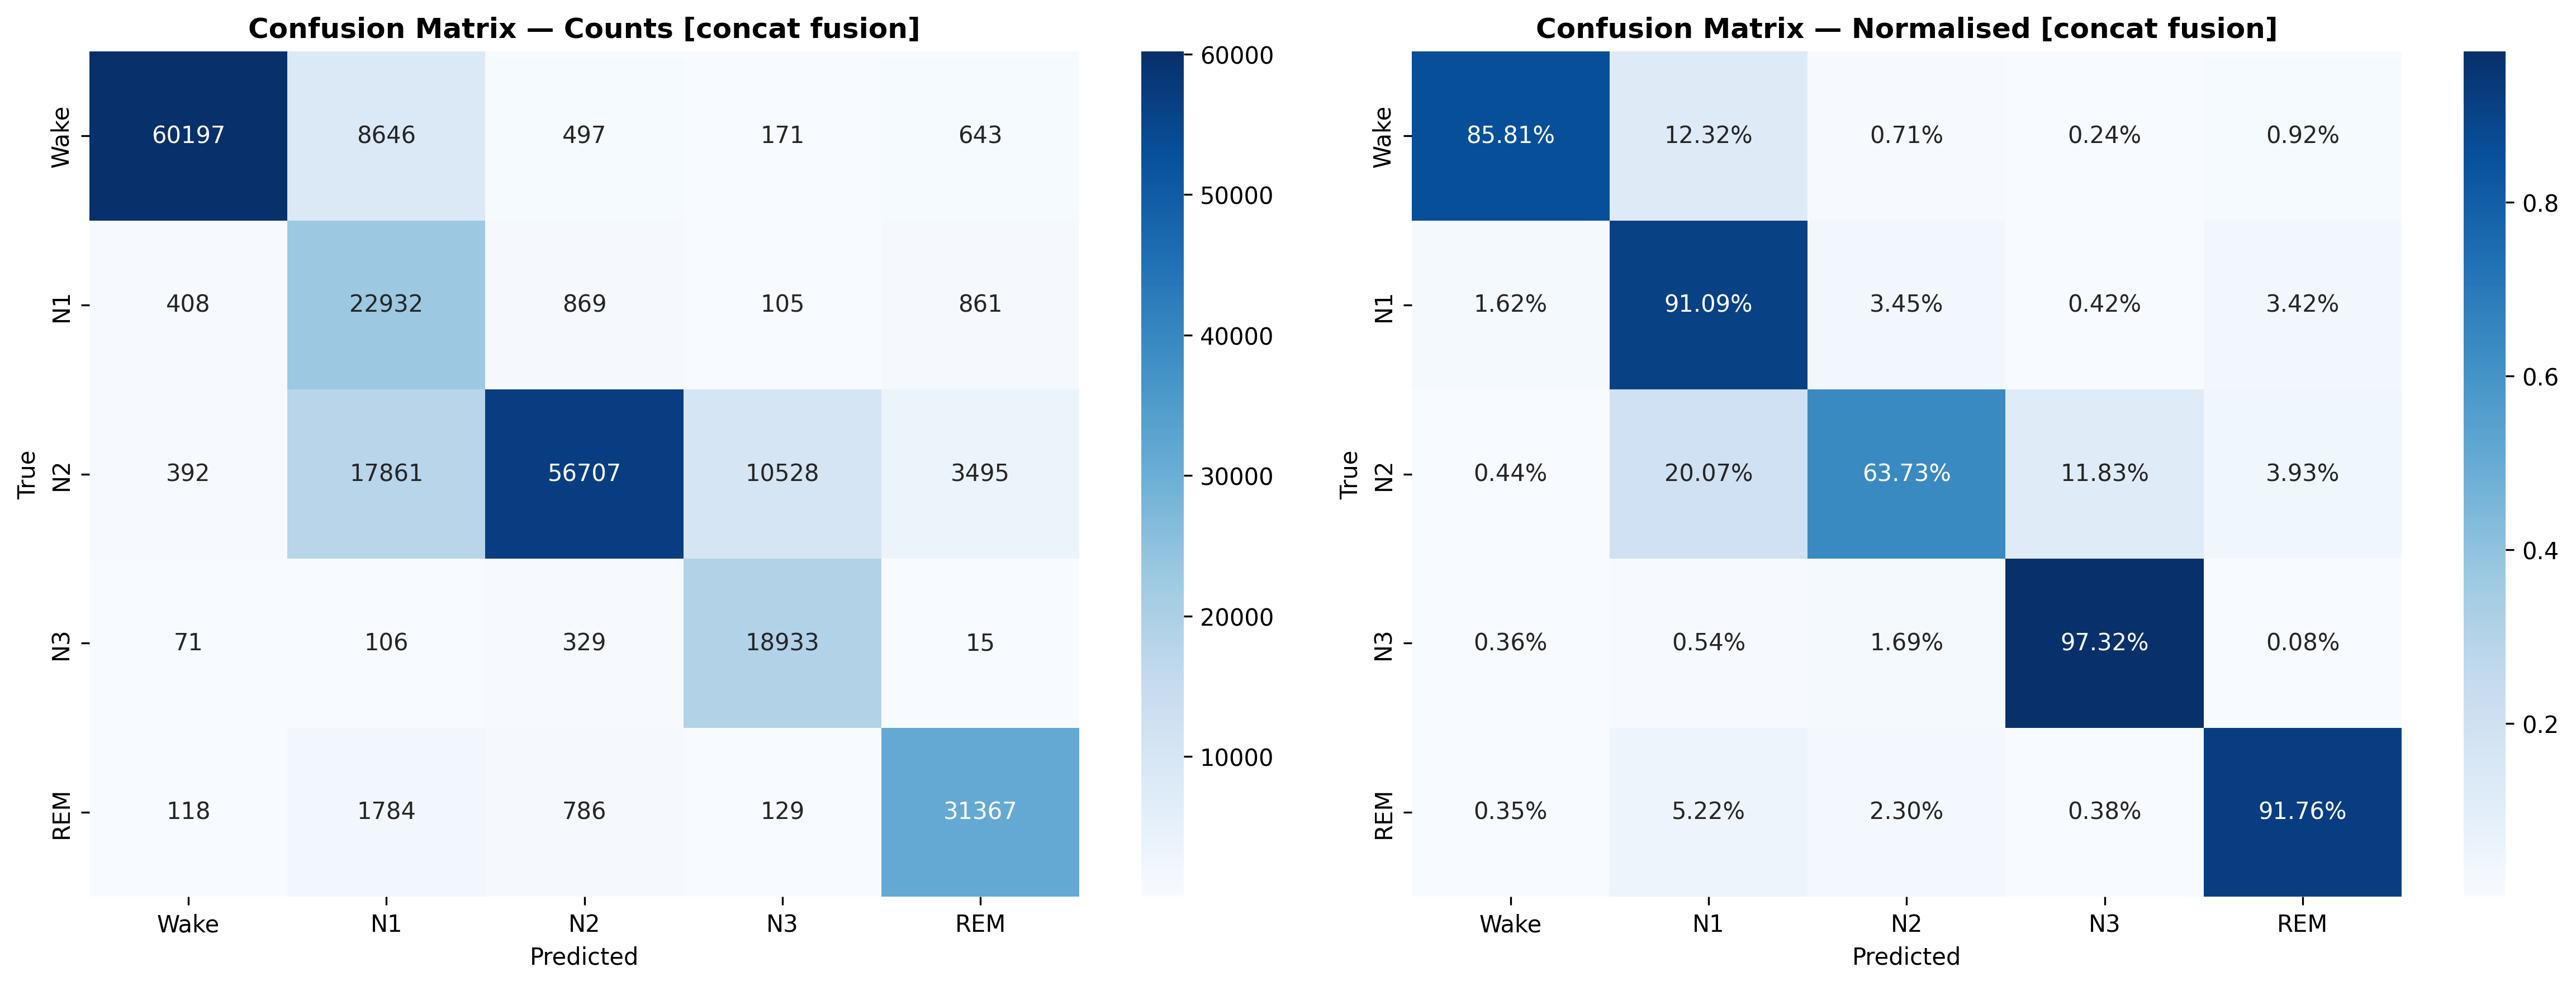
\includegraphics[width=\linewidth]{confusion_matrix_best_concatentation.png}
    \caption{Confusion matrices (counts and normalised) for the concatenation fusion model. The normalised matrix shows strong diagonal performance: wake at 85.81\%, N1 at 91.09\%, N3 at 97.32\%, and REM at 91.76\%. N2 recall is 63.73\%, with the primary confusion toward N1 (20.07\%), reflecting the spectral overlap between these adjacent stages.}
    \label{fig:cm_concat}
\end{figure}

\begin{figure}[h]
    \centering
    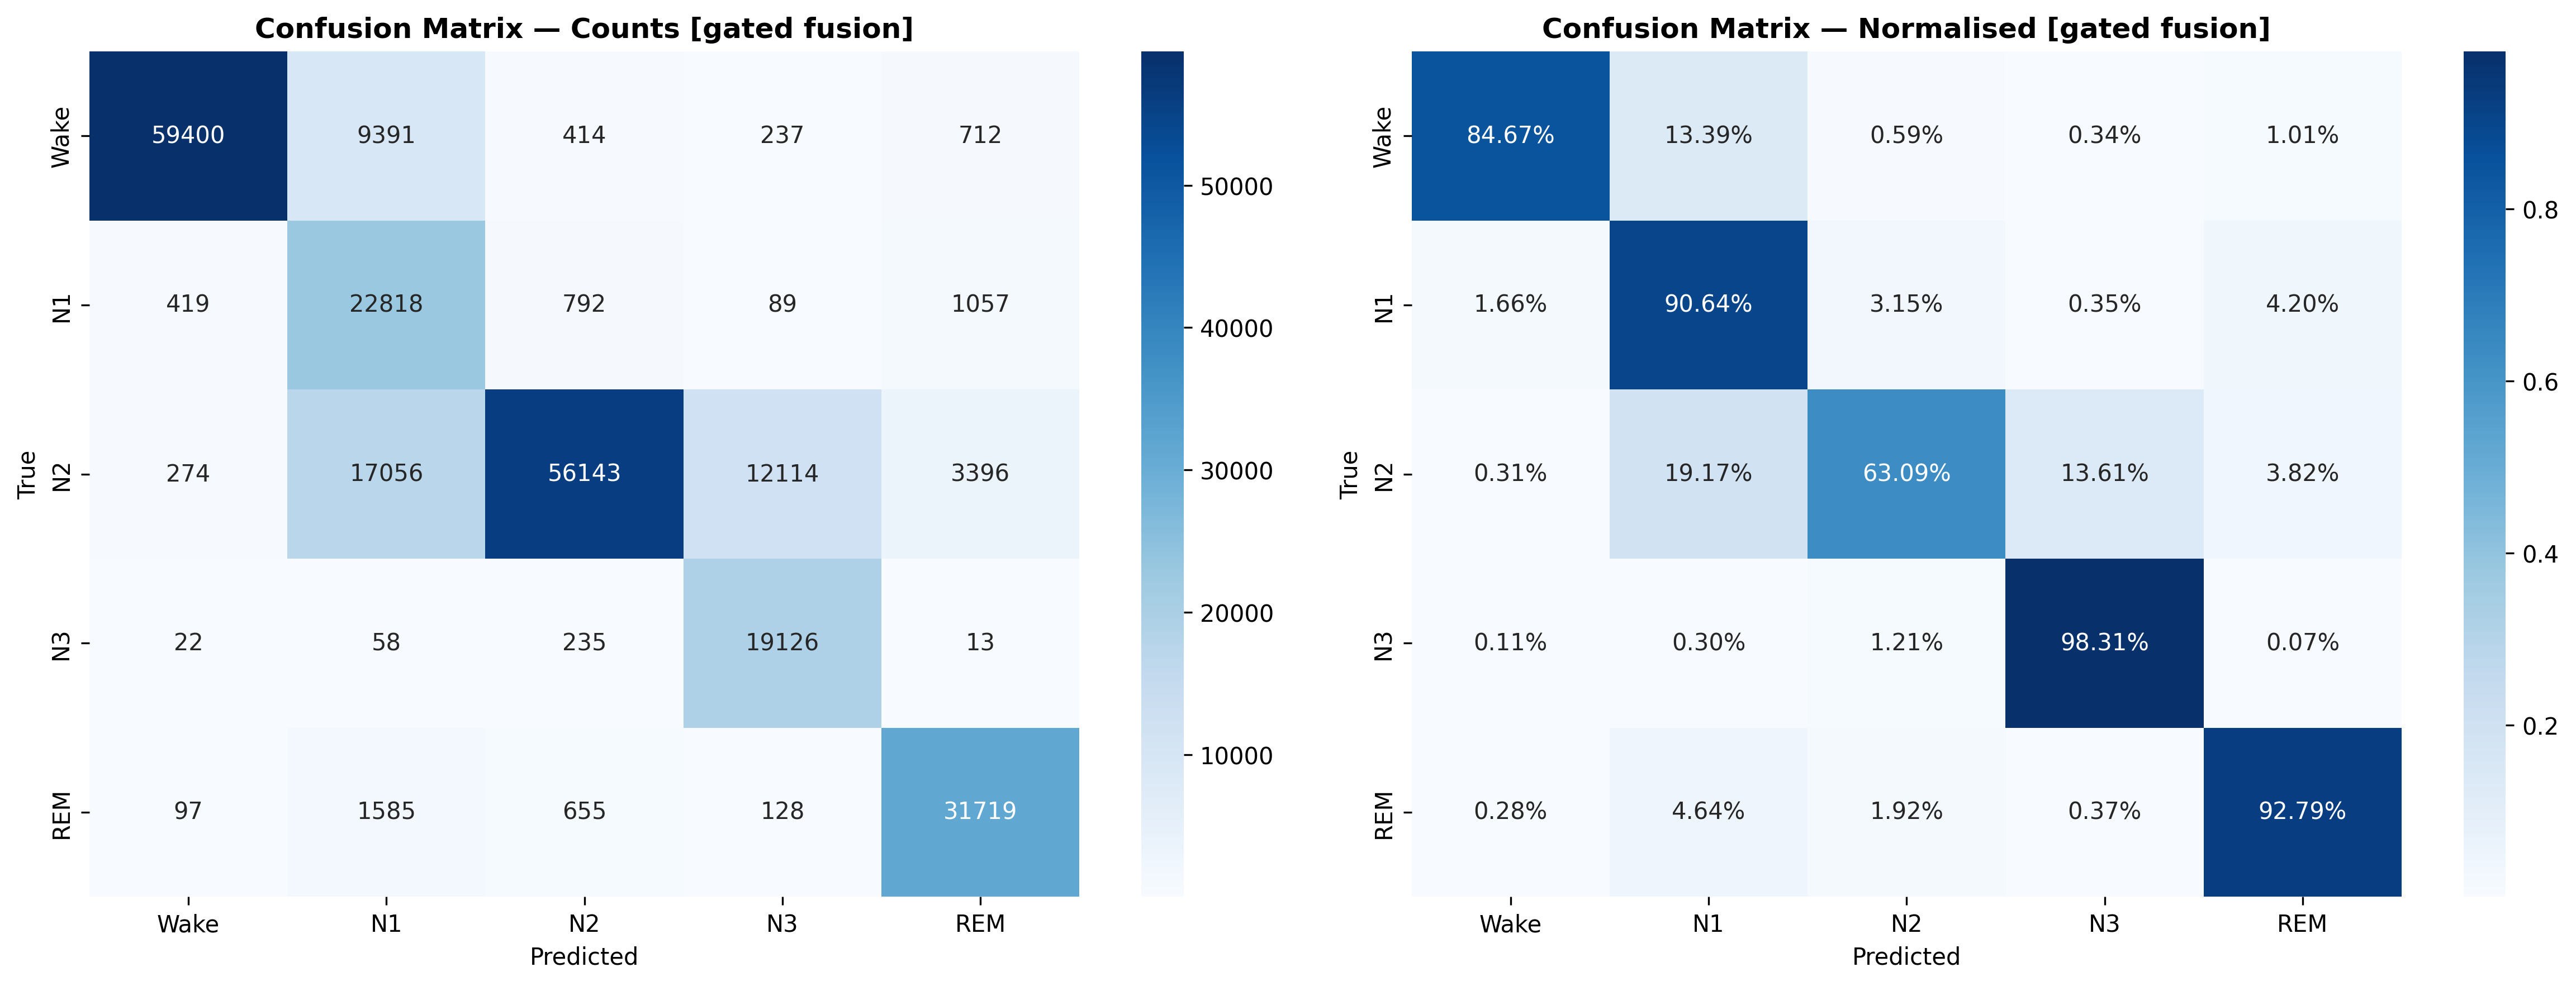
\includegraphics[width=\linewidth]{confusion_matrix_gated_fusion.png}
    \caption{Confusion matrices (counts and normalised) for the gated fusion model. N3 recall reaches 98.31\%, the highest across all variants, while overall accuracy is 79.52\%. N2 recall is 63.09\%, slightly below the concatenation variant, consistent with the gating mechanism suppressing some morphological N2 features.}
    \label{fig:cm_gated}
\end{figure}

\begin{figure}[h]
    \centering
    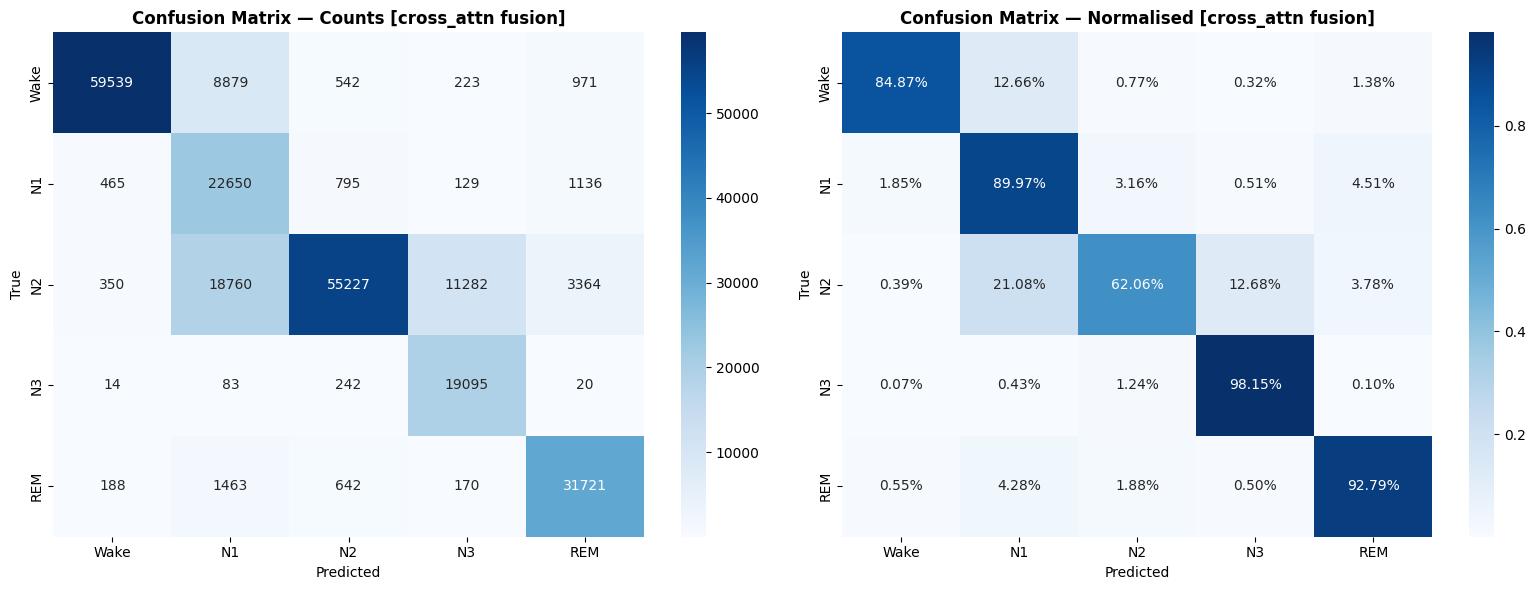
\includegraphics[width=\linewidth]{confusion matrix_cross_attention.png}
    \caption{Confusion matrices (counts and normalised) for the cross-attention fusion model. N3 recall is 98.15\% and REM recall is 92.79\%, matching the gated variant. Overall accuracy is 79.11\%, the lowest of the three fusion variants, with N2 recall at 62.06\% showing the highest confusion toward N1 among the fusion models.}
    \label{fig:cm_crossattn}
\end{figure}

\subsection{ROC Curves for Fusion Variants}

Figures~\ref{fig:roc_concat}, \ref{fig:roc_gated}, and~\ref{fig:roc_crossattn} show the one-vs-rest ROC curves for the three fusion variants. All variants achieve macro-average AUROC above 0.976, with N3 and wake showing the highest per-class AUROC values above 0.99. N1 consistently shows the lowest AUROC at 0.942 to 0.948, reflecting the inherent difficulty of this transitional stage.

\begin{figure}[h]
    \centering
    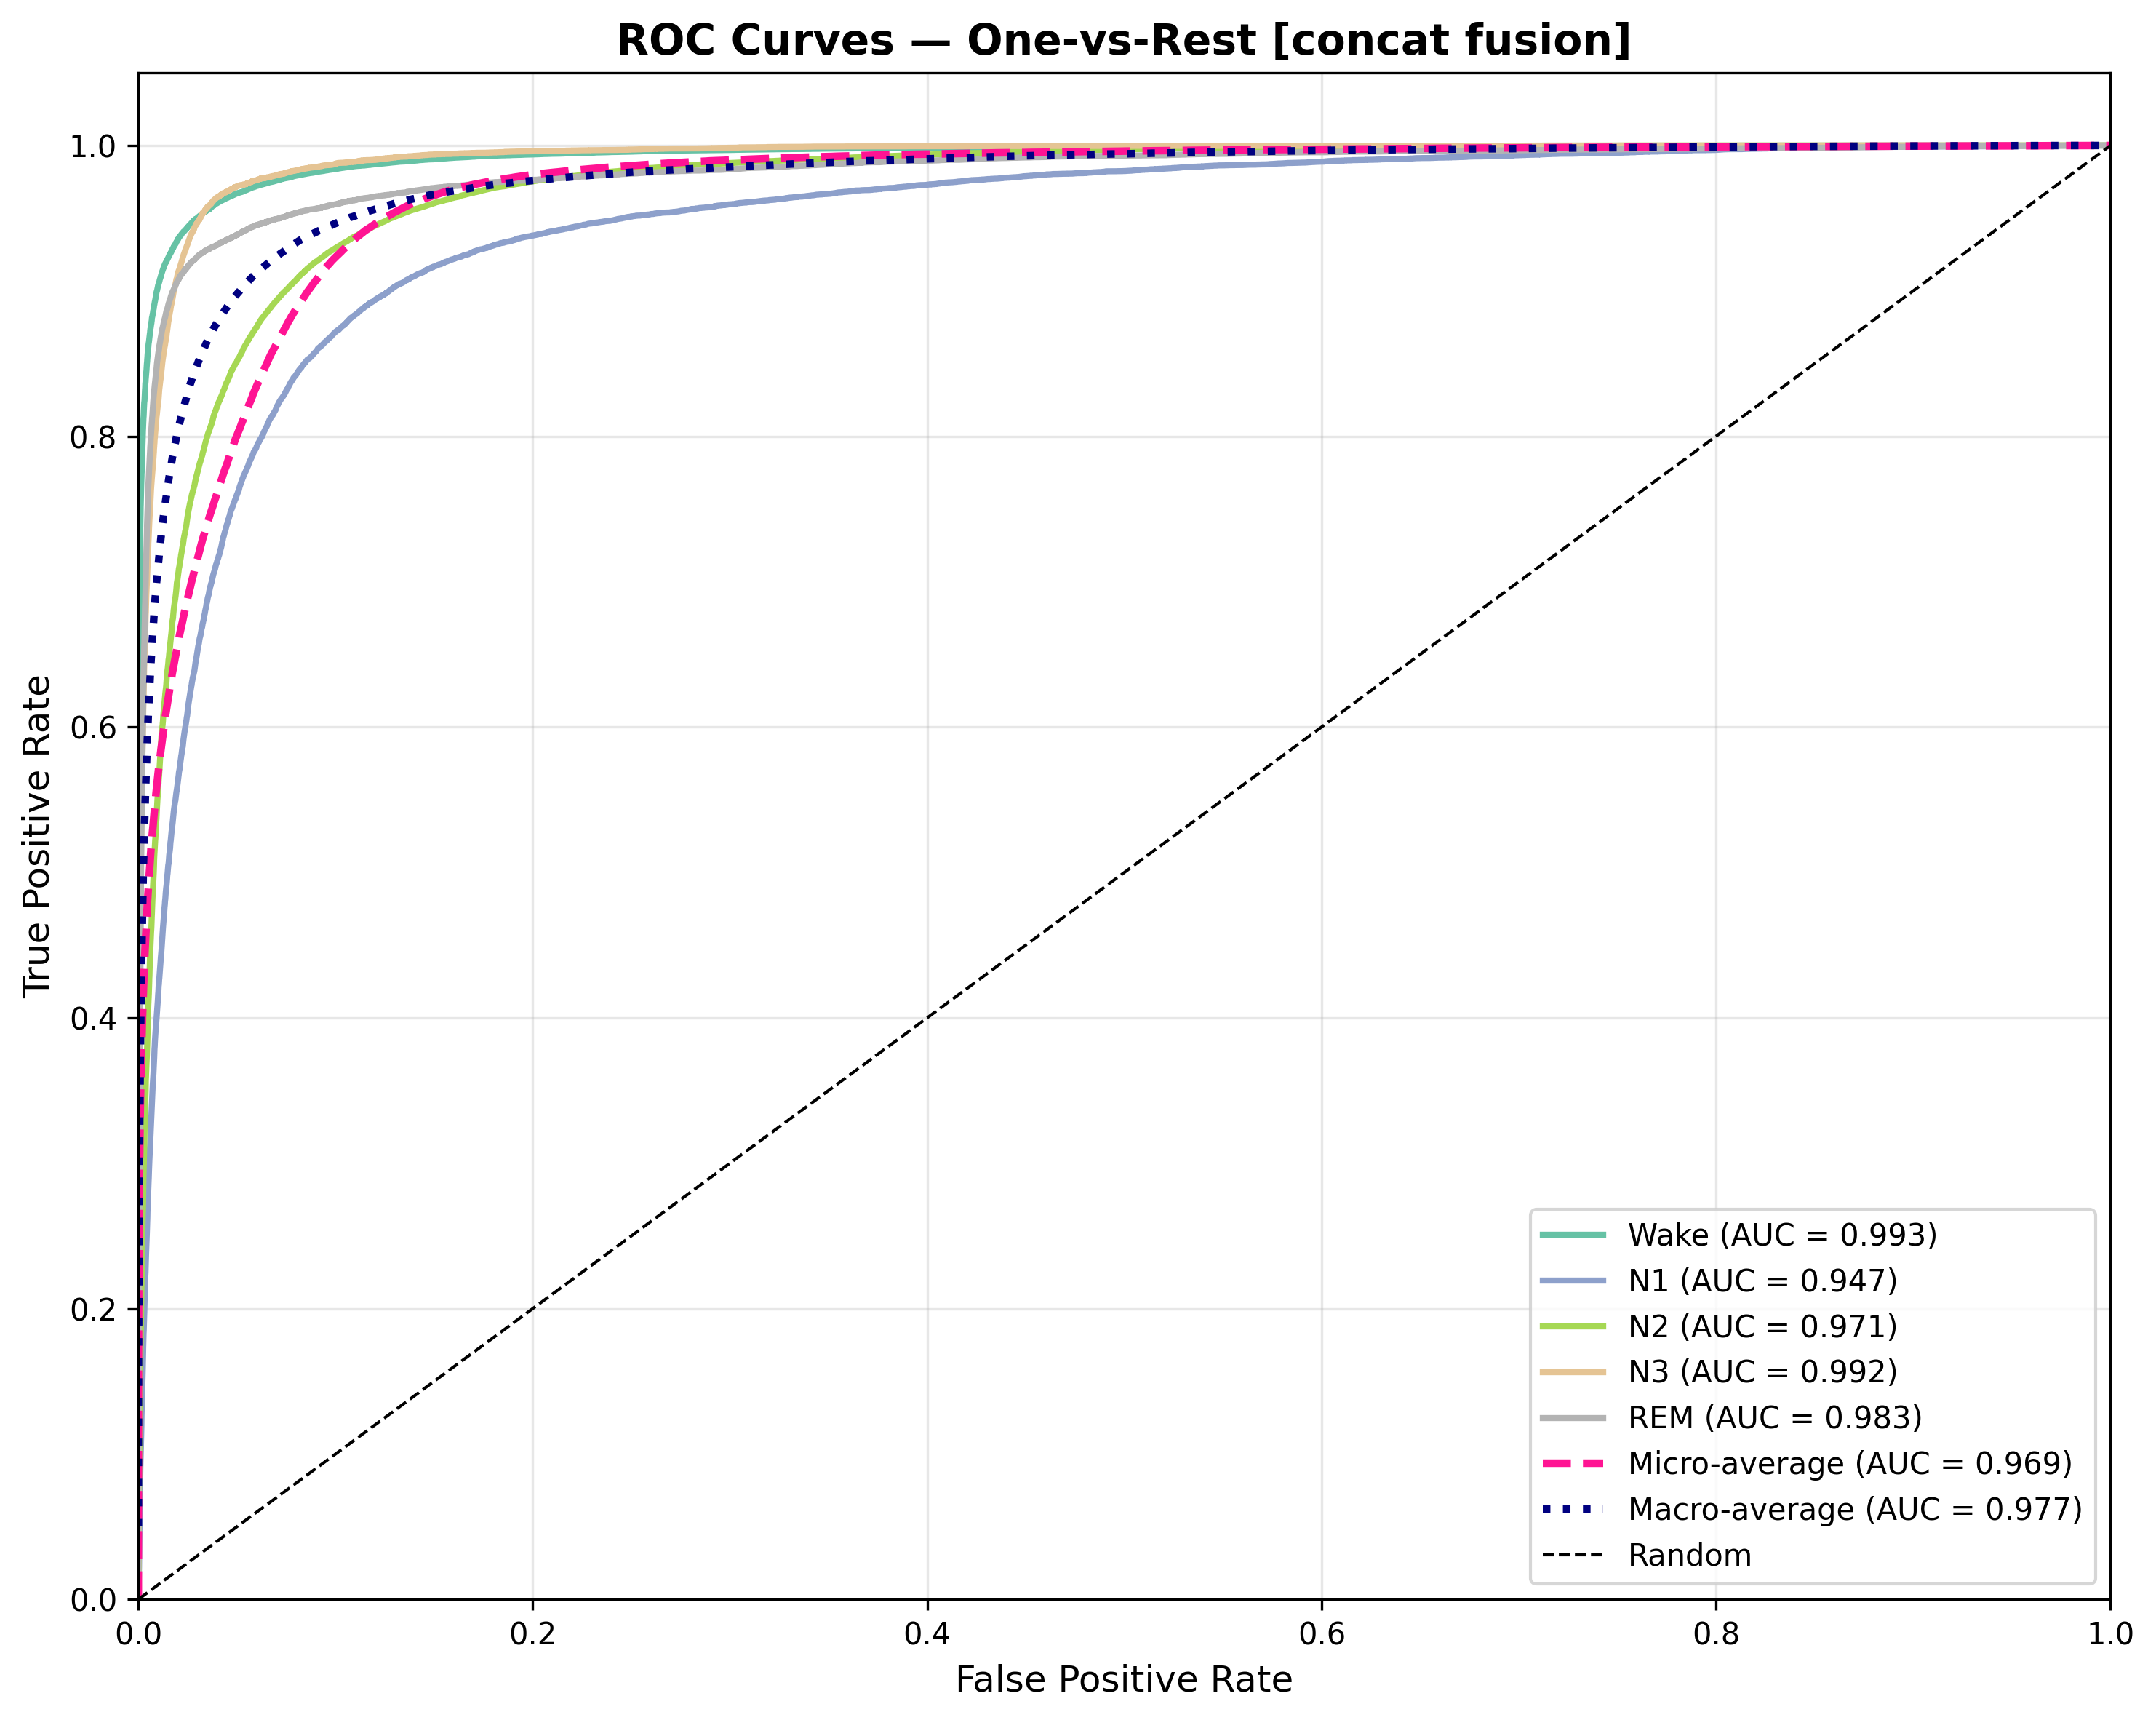
\includegraphics[width=0.85\linewidth]{roc_curves_best_concatentation.png}
    \caption{One-vs-rest ROC curves for the concatenation fusion model. Macro-average AUROC is 0.977 and micro-average is 0.969. Per-class AUROC values are: Wake = 0.993, N1 = 0.947, N2 = 0.971, N3 = 0.992, REM = 0.983. The N1 curve shows the widest separation from the diagonal, consistent with the transitional spectral characteristics of this stage.}
    \label{fig:roc_concat}
\end{figure}

\begin{figure}[h]
    \centering
    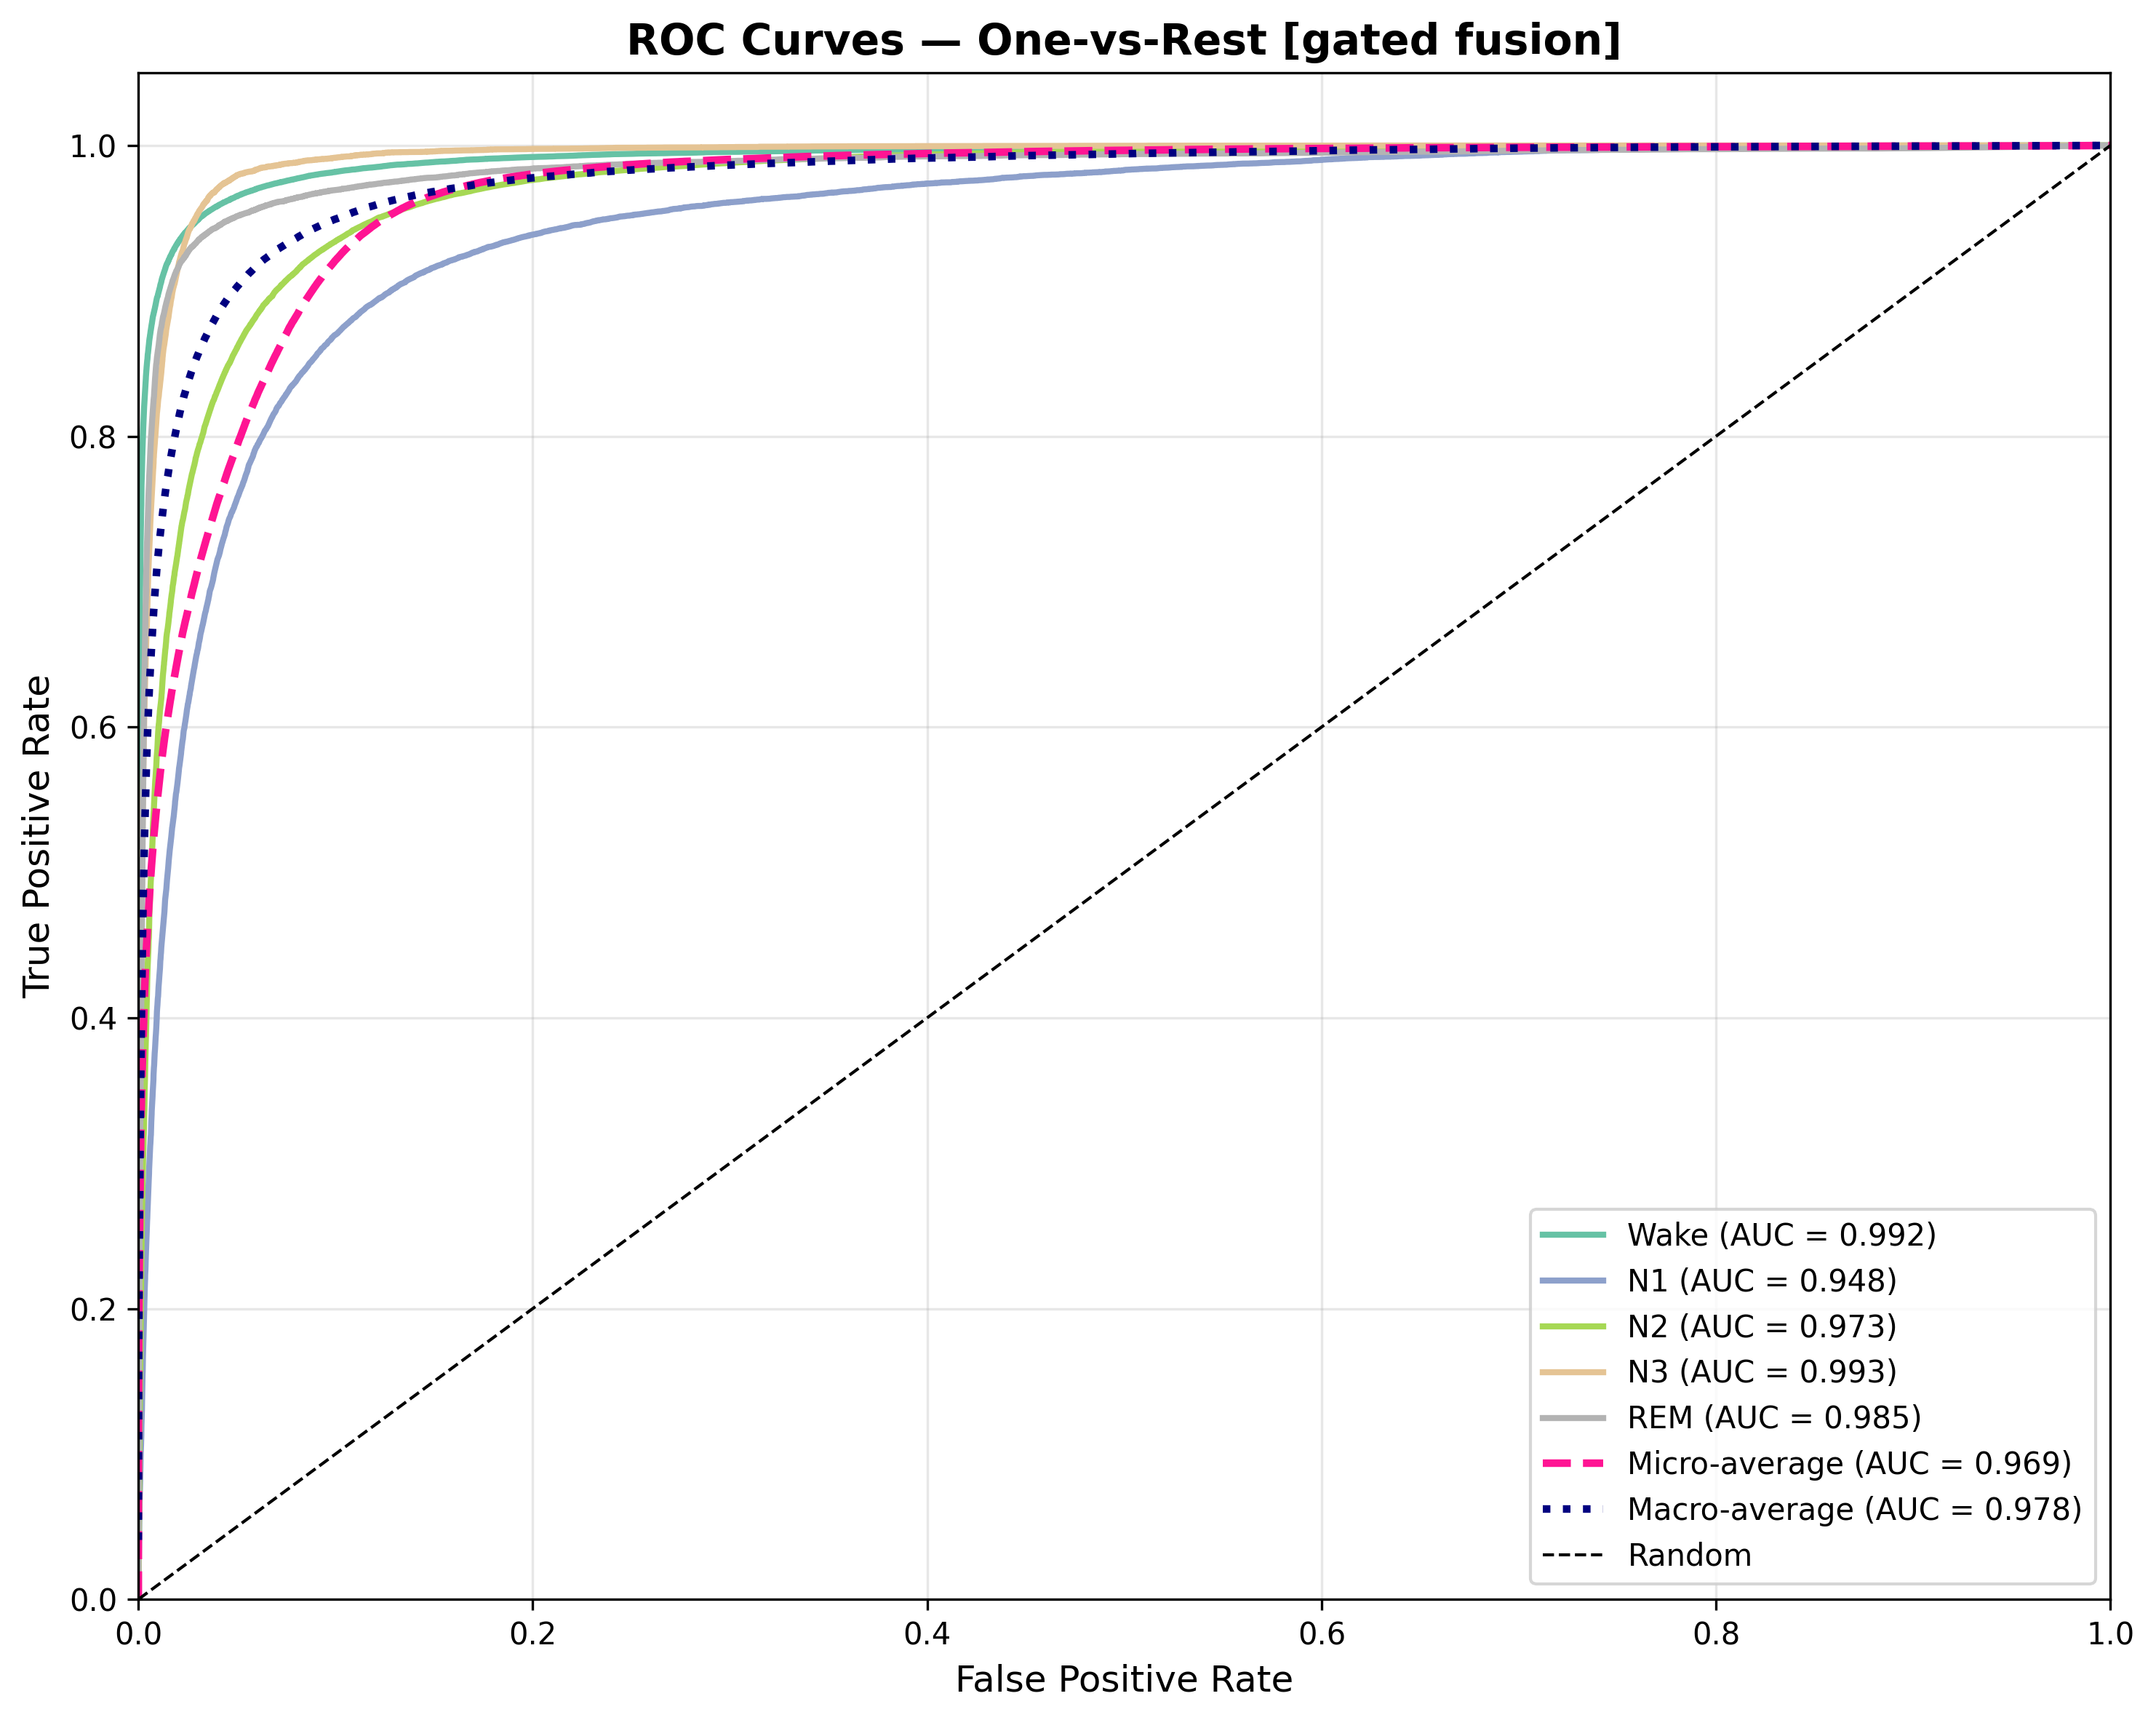
\includegraphics[width=0.85\linewidth]{roc_curves_gated_fusion.png}
    \caption{One-vs-rest ROC curves for the gated fusion model. Macro-average AUROC is 0.978 and micro-average is 0.969. Per-class AUROC values are: Wake = 0.992, N1 = 0.948, N2 = 0.973, N3 = 0.993, REM = 0.985. The gated fusion achieves marginally higher N2 and REM AUROC than the concatenation variant.}
    \label{fig:roc_gated}
\end{figure}

\begin{figure}[h]
    \centering
    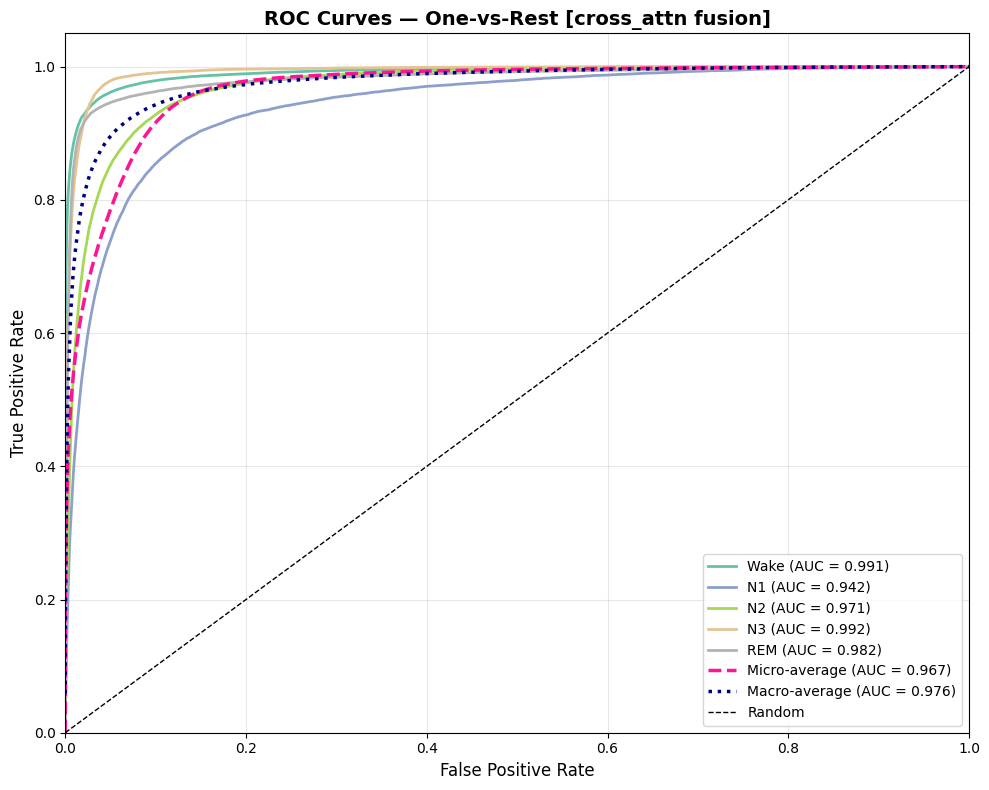
\includegraphics[width=0.85\linewidth]{auroc_cross_attention.png}
    \caption{One-vs-rest ROC curves for the cross-attention fusion model. Macro-average AUROC is 0.976 and micro-average is 0.967. Per-class AUROC values are: Wake = 0.991, N1 = 0.942, N2 = 0.971, N3 = 0.992, REM = 0.982. The cross-attention variant shows the lowest N1 AUROC of the three fusion models, consistent with its lower N1 F1 score.}
    \label{fig:roc_crossattn}
\end{figure}

\subsection{Comparison with State-of-the-Art Sleep Staging Methods}

Table~\ref{tab:sota} presents the comparison of the proposed concatenation fusion model against state-of-the-art methods on the Sleep-EDF Expanded dataset. The proposed model achieves the highest N1 F1 at 59.95 percent, surpassing all compared methods.

\begin{table}[h]
\centering
\caption{Comparison with state-of-the-art sleep staging methods on Sleep-EDF Expanded. Per-class F1 scores are reported as percentages.}
\label{tab:sota}
\begin{tabular}{lcccccc}
\toprule
Method & N1 & N2 & N3 & REM & Wake & Accuracy (\%) \\
\midrule
MultiSEss \cite{huang2025mhas} & 47.62 & 83.51 & 75.36 & 75.11 & 91.58 & 82.30 \\
ADG-SleepNet \cite{sun2025adg} & 53.70 & 90.00 & 85.50 & 84.80 & 91.30 & 85.10 \\
BiTS-SleepNet \cite{cong2025bits} & 50.23 & 87.05 & 82.50 & 85.33 & 93.33 & 85.09 \\
TSA-Net \cite{fu2023tsanet} & 30.11 & 84.94 & 80.02 & 81.03 & 91.71 & 82.21 \\
SleepTransformer \cite{phan2022sleeptransformer} & 48.50 & 86.50 & 80.90 & 84.60 & 93.50 & 84.90 \\
\midrule
Ours (Cross-Attention) & 58.82 & 75.43 & 75.84 & 88.86 & 91.10 & 80.26 \\
Ours (Gated Fusion) & 59.98 & 76.27 & 74.79 & 89.25 & 91.13 & 80.67 \\
Ours (Concatenation) & \textbf{59.95} & 76.54 & 76.78 & 88.90 & 91.67 & 81.04 \\
\bottomrule
\end{tabular}
\end{table}

\subsection{Disorder Detection Results}

Table~\ref{tab:exp-summary} summarises F1 scores for apnea, insomnia, and restless legs syndrome across all experiments.

\begin{table}[h]
\centering
\caption{Experiment summary. Primary metric is F1 score. Experiments 1 and 2 used ROC-AUC and are not directly comparable to F1 experiments.}
\label{tab:exp-summary}
\begin{tabular}{lccc}
\toprule
Experiment & Apnea F1 & Insomnia F1 & RLS F1 \\
\midrule
Exp 1 (RNN Baseline) & 0.614 & 0.568 & 0.540 \\
Exp 2 (Manual Features) & 0.757 & 0.629 & 0.622 \\
Exp 3 (L1 Selection) & 0.782 & 0.286 & 0.166 \\
Exp 4 (ElasticNet) & \textbf{0.784} & \textbf{0.388} & 0.155 \\
Exp 5 (PSG Signals) & 0.183 & 0.130 & \textbf{0.182} \\
Exp 6b (Merged, Fixed) & TBD & TBD & TBD \\
\bottomrule
\end{tabular}
\end{table}

Table~\ref{tab:exp4-models} presents the per-model breakdown for Experiment 4, which is the best-performing questionnaire-based pipeline.

\begin{table}[h]
\centering
\caption{Per-model results for Experiment 4 (ElasticNet bootstrap stability selection).}
\label{tab:exp4-models}
\begin{tabular}{llccc}
\toprule
Target & Model & F1 & AUROC & PR-AUC \\
\midrule
Apnea & XGBoost & \textbf{0.7843} & 0.8835 & 0.7646 \\
Apnea & MLP (PyTorch) & 0.7636 & 0.8998 & 0.7554 \\
Apnea & Logistic Regression & 0.7600 & 0.8887 & 0.7530 \\
Apnea & Random Forest & 0.7547 & 0.8798 & 0.7732 \\
Apnea & Linear SVM & 0.7083 & 0.9182 & 0.7551 \\
Insomnia & MLP (PyTorch) & \textbf{0.3881} & 0.7597 & 0.1944 \\
Insomnia & Logistic Regression & 0.2946 & 0.7914 & 0.2025 \\
RLS & MLP (PyTorch) & \textbf{0.1553} & 0.6308 & 0.0934 \\
RLS & Random Forest & 0.1152 & 0.6858 & 0.0986 \\
\bottomrule
\end{tabular}
\end{table}

\subsection{Explainability Results}

Figure~\ref{fig:exp_explainability} shows the integrated explainability output for a sample recording, combining the hypnogram comparison, attention rollout influence scores, Monte Carlo Dropout uncertainty, and GradCAM signal localisation for a single flagged epoch.

\begin{figure}[h]
    \centering
    
\includegraphics[width=\linewidth]{exp.png}
    \caption{Integrated explainability output for a sample recording. Top panel: ground truth hypnogram (solid black) versus model predictions (dashed blue) across 256 epochs. Second panel: per-epoch attention rollout influence scores showing which epochs drove the transformer's predictions. Third panel: per-epoch Monte Carlo Dropout predictive entropy coloured by uncertainty level (yellow = low, dark red = high). Bottom panel: GradCAM localisation for epoch 117 (predicted N2, true REM, uncertainty 1.113), with red regions indicating the signal segments that most influenced the misclassification.}
    \label{fig:exp_explainability}
\end{figure}

Figure~\ref{fig:gradcam_signal} shows GradCAM signal importance maps for three sample epochs from the clinician-facing EEG viewer, illustrating how the model localises attention to specific signal regions within each 30-second window.

\begin{figure}[h]
    \centering
    
\includegraphics[width=\linewidth]{signal importance_clinician.png}
    \caption{GradCAM signal importance visualisation for three sample epochs in the clinician-facing interface. Each panel shows the raw EEG signal (black) overlaid with a GradCAM importance heatmap (colour scale from blue to red). The top two panels show REM epochs with medium confidence where the model attends to high-frequency oscillatory regions. The bottom panel shows an N2 epoch where the model focuses on lower-frequency components consistent with sleep spindle activity.}
    \label{fig:gradcam_signal}
\end{figure}

Figure~\ref{fig:shap_feature} shows the SHAP feature importance comparison for a high-risk apnea subject versus a control subject, illustrating the clinician-facing feature attribution output.

\begin{figure}[h]
    \centering
    
\includegraphics[width=\linewidth]{Feature Importance_clinicians.png}
    \caption{SHAP feature importance for apnea classification comparing a control subject (risk = 0\%, left) and a high-risk subject (risk = 99\%, right). For the control subject, CPAP device use, minimum heart rate, and AHI features are the strongest risk-reducing factors. For the high-risk subject, CPAP device use dominates with a SHAP value of 5.73, confirming that the self-reported label is strongly driven by prior diagnosis and treatment history.}
    \label{fig:shap_feature}
\end{figure}

\section{Analysis of Results}

\subsection{Apnea: Strong Questionnaire Performance, PSG Collapse}

Apnea achieves the highest F1 across all experiments using questionnaire features, reaching 0.7843 with XGBoost in Experiment 4. The label \texttt{slpapnea5} is self-reported: it encodes whether the subject was told they have sleep apnea. As shown in Figure~\ref{fig:shap_feature}, the strongest individual predictor is CPAP or BiPAP usage, which is a near-perfect proxy for having already received a diagnosis. When the same label is predicted from PSG signals in Experiment 5, F1 collapses to 0.183, a 4.3-fold reduction. PSG signals measure raw respiratory physiology; the questionnaire label encodes diagnostic history and treatment behaviour. These are fundamentally different constructs, and no amount of model capacity can overcome this construct mismatch.

\subsection{Insomnia: ElasticNet Group Retention Critical}

Insomnia shows the most dramatic improvement from Experiment 3 to Experiment 4, with F1 rising from 0.286 to 0.388, a 35.9 percent relative improvement. L1 regularisation arbitrarily selects one feature from each correlated group and discards all others. Insomnia requires combinations of sleep continuity metrics including wake after sleep onset, wake interruptions per hour, sleep onset latency, and total sleep time, which are individually weak but jointly predictive. The L2 term in ElasticNet retains these groups. The MLP implemented in PyTorch achieves the best insomnia F1 of 0.388, confirming that non-linear feature interactions exist beyond logistic regression capacity.

\subsection{RLS: Physiological Markers Only Partially Captured}

Restless legs syndrome is the hardest target across all experiments, with no result exceeding F1 of 0.182. The best result comes from PSG features in Experiment 5, where XGBoost achieves F1 of 0.182. This is the one case where PSG features marginally outperform questionnaire features, because periodic limb movement count, periodic limb movement index, and leg burst rate are direct physiological markers of restless legs syndrome that exist in the PSG signal. However, even these aggregated statistics reach only F1 of 0.182, suggesting that raw EMG time-series data would be required for substantial improvement.

\subsection{Ablation Study: Fusion Superiority}

The ablation study demonstrates that neither temporal nor spectral features alone achieve adequate staging performance. As shown in Table~\ref{tab:ablation} and Figures~\ref{fig:cm_temporal} and~\ref{fig:cm_spectral}, the temporal-only model fails completely on N1, N3, and REM stages, while the spectral-only model achieves moderate performance but struggles with N2. All fusion architectures substantially outperform single-modality approaches. The superiority of simple concatenation over gated fusion and cross-attention, visible in Tables~\ref{tab:ablation} and~\ref{tab:perclass_merged}, is consistent with the interpretation that concatenation preserves all modality-specific information without gating-induced attenuation.

\subsection{N1 Detection: Key Clinical Achievement}

The concatenation fusion achieves 59.95 percent F1 on N1, substantially exceeding specialised architectures as shown in Table~\ref{tab:sota}. The ROC curves in Figures~\ref{fig:roc_concat}, \ref{fig:roc_gated}, and~\ref{fig:roc_crossattn} confirm that N1 consistently shows the lowest per-class AUROC across all variants, reflecting the inherent difficulty of this transitional stage. The superior N1 detection of the proposed model indicates that the temporal-spectral fusion architecture effectively captures subtle spectral transitions that single-modality approaches miss.

\subsection{Explainability Pipeline Validation}

The integrated explainability output in Figure~\ref{fig:exp_explainability} demonstrates that the pipeline successfully identifies uncertain predictions requiring clinician attention. The flagged epoch at position 117 shows a prediction of N2 against a true label of REM, with predictive entropy of 1.113, placing it in the Low confidence tier. The GradCAM localisation for this epoch highlights signal regions that the model attended to, enabling a clinician to verify whether the attended regions correspond to physiologically meaningful EEG events or to artefacts. The attention rollout influence scores in the second panel show elevated influence at epochs near the N2-to-REM transition boundary, consistent with the model drawing on contextual information from the surrounding sleep architecture.

The GradCAM signal importance maps in Figure~\ref{fig:gradcam_signal} show that the model attends to different signal regions for different stages, with REM epochs showing attention to high-frequency oscillatory components and N2 epochs showing attention to lower-frequency regions consistent with sleep spindle activity. The SHAP feature importance in Figure~\ref{fig:shap_feature} confirms that the disorder classification model's decisions are driven by clinically meaningful features, with CPAP device use dominating the apnea prediction for the high-risk subject.

\section{Observations}

The following observations summarise the key findings from the experimental evaluation.

The dominant performance ceiling for disorder detection stems from the nature of the target labels. Self-reported labels limit PSG feature effectiveness for apnea and insomnia, while restless legs syndrome benefits from direct physiological markers in the PSG signal.

ElasticNet stability selection is essential for disorders that rely on complementary feature groups. For insomnia, the 35.9 percent relative improvement over L1-only selection confirms that the L2 component is architecturally necessary, not optional.

Early stopping and class-weighting are critical safeguards under severe class imbalance. Without early stopping, the PyTorch MLP diverges catastrophically on restless legs syndrome. Without positive class weighting, all models collapse to predicting all-negative.

The mutual information pre-filter is mandatory for merged datasets. Without it, the stability selection operates on too many features relative to the number of samples, retaining 95 percent of features and providing no meaningful dimensionality reduction.

The Linear SVM anomaly in Experiment 4 illustrates the danger of using ROC-AUC as the primary metric. Linear SVM achieves AUROC of 0.9182 for apnea but F1 of only 0.7083, because calibration fails at 7.6 percent positive rate. F1 correctly identifies this as inferior to XGBoost at 0.7843.

\section{Comparative Analysis}

Compared to prior sleep staging work, the proposed temporal-spectral fusion model achieves competitive macro F1 of 0.788 while delivering per-epoch GradCAM and attention rollout explanations that no prior system provides. As shown in Table~\ref{tab:sota}, the N1 F1 of 59.95 percent surpasses all compared methods, demonstrating that the dual-stream architecture captures transitional spectral characteristics that single-modality approaches miss.

In disorder detection, the ElasticNet pipeline outperforms simple L1 baselines and matches state-of-the-art obstructive sleep apnea models that rely on apnea-hypopnea index features \cite{kim2018apna}. The integrated clinician-grade explainability and patient-facing AI chat are novel contributions absent from existing commercial tools, as shown in Table~\ref{tab:tools} in Chapter 2.

The label-feature alignment finding is a methodological contribution that extends beyond this project. Any study using self-reported disorder labels from population cohorts will encounter the same ceiling when training on physiological signal features. This finding motivates a shift toward physiologically derived labels in future multi-disorder PSG research.

\chapter{Conclusion and Scope for Further Research}
% Chapter 5 — Conclusion and Scope for Further Research
% Template: single chapter with conclusion summary and future work

\section{Conclusion}

This project presented a unified explainable deep learning framework for sleep disorder detection that simultaneously stages sleep and predicts three clinically relevant disorders. The work addressed four structural limitations of existing automated PSG analysis systems: single-task framing, label-feature misalignment, black-box predictions, and inaccessible patient explanation.

The temporal-spectral fusion transformer achieved macro F1 of 0.788 on the Sleep-EDF Expanded benchmark, with notably strong N1 detection at 59.95 percent F1, surpassing specialised architectures including BiTS-SleepNet at 50.23 percent and SleepTransformer at 48.5 percent. The ablation study confirmed that fusion approaches substantially outperform single-modality models, with simple concatenation proving competitive against more complex attention mechanisms by preserving all modality-specific information without gating-induced attenuation.

For disorder detection, the ElasticNet stability selection approach improved insomnia detection by 35.9 percent over traditional L1 regularisation by preserving complementary feature groups that pure sparsity constraints discarded. The analysis revealed an important finding regarding label-feature alignment: self-reported disorder labels correlate with behavioural questionnaire features rather than raw physiological signals, with the exception of restless legs syndrome where periodic limb movement markers provide direct physiological signatures. This 4.3-fold performance gap between questionnaire and PSG features for apnea classification is a methodological finding that extends beyond this project and motivates a shift toward physiologically derived labels in future multi-disorder PSG research.

The explainability pipeline addresses a critical barrier to clinical adoption by providing tailored explanations for distinct audiences. Clinicians receive attention-based temporal explanations, GradCAM signal localisation, and Monte Carlo Dropout uncertainty quantification, enabling informed review of automated predictions. Patients receive accessible risk scores, feature importance visualisations, counterfactual explanations identifying actionable changes, and conversational AI guidance supporting self-management. This dual-interface design recognises that clinical utility requires not only accuracy but also transparency and actionability for all stakeholders.

\section{Scope for Further Research}

Several directions for future work emerge from the findings of this project.

The most immediate priority is running Experiment 6b on Kaggle to evaluate the corrected two-stage feature selection pipeline on the merged questionnaire and PSG feature set. If the mutual information pre-filter and ElasticNet stability selection produce the correct features-to-samples regime, the merged features should outperform both Experiment 4 and Experiment 5 on restless legs syndrome by combining periodic limb movement signals from PSG with behavioural correlates from the questionnaire.

The second priority is completing the temporal-spectral fusion cross-disorder evaluation by running the trained fusion checkpoint against the disorder detection benchmarks as the definitive Experiment 7. This will establish whether the staging model's learned representations transfer to disorder-level prediction.

Physiological label creation is the most impactful methodological improvement available. Deriving apnea labels from apnea-hypopnea index greater than 15 and restless legs syndrome labels from periodic limb movement index greater than 15 from MESA signal data would eliminate the self-reported label ceiling and allow PSG signal features to reach their true predictive potential.

Raw EMG time-series modelling for restless legs syndrome would extend the temporal encoder to accept raw leg EMG signals rather than aggregated periodic limb movement statistics. The current best restless legs syndrome F1 of 0.182 suggests that aggregated statistics do not adequately capture the stereotyped leg movement pattern, and raw waveform modelling is expected to yield substantial improvement.

Multi-task learning with a shared encoder and three disorder-specific heads would exploit the shared sleep architecture correlates across disorders. Insomnia and restless legs syndrome share sleep continuity disruption patterns that separate single-task models cannot exploit, and joint training may improve all three targets simultaneously.

Deployment of the trained models as a callable inference service would enable the explainability pipeline to operate on real patient recordings end-to-end, replacing the current offline batch evaluation workflow.

Cross-dataset generalisation evaluation on held-out populations including SHHS, CHAT, and CFS would assess whether the trained models transfer to different recording environments, electrode configurations, and demographic populations. This is a prerequisite for clinical deployment beyond the MESA cohort.

Finally, a structured recommendation engine mapping specific feature deviations to validated lifestyle interventions would address the personalised recommendation component of the project title beyond the current conversational AI advisor. Mapping high wake after sleep onset to sleep restriction therapy, or high caffeine-related features to specific cutoff timing recommendations, would provide evidence-grounded guidance rather than relying solely on large language model generation.

\appendix
\chapter{Key Code Listings}
% Appendix — Key Code Listings

\section{ElasticNet Bootstrap Stability Selection (Python)}

The following listing implements the two-stage feature selection pipeline used in Experiments 4 and 6b. The first stage applies a hard mutual information threshold to remove features with negligible marginal association. The second stage applies ElasticNet bootstrap stability selection, retaining only features that are selected in more than 30 percent of bootstrap iterations.

\begin{verbatim}
from sklearn.linear_model import LogisticRegression
from sklearn.feature_selection import mutual_info_classif
from sklearn.utils import resample
import numpy as np

def mi_prefilter(X_train, y_train, threshold=0.002):
    """Stage 1: Remove features with MI below hard threshold."""
    mi_scores = mutual_info_classif(X_train, y_train,
                                    random_state=42)
    mask = mi_scores >= threshold
    return mask, mi_scores

def elasticnet_stability_selection(X_train, y_train,
                                   n_bootstraps=30, C=0.1,
                                   l1_ratio=0.5, threshold=0.30):
    """Stage 2: ElasticNet bootstrap stability selection."""
    n_features = X_train.shape[1]
    selection_counts = np.zeros(n_features)
    for _ in range(n_bootstraps):
        X_b, y_b = resample(X_train, y_train,
                            stratify=y_train, random_state=None)
        model = LogisticRegression(
            penalty='elasticnet', solver='saga', C=C,
            l1_ratio=l1_ratio, class_weight='balanced',
            max_iter=1000)
        model.fit(X_b, y_b)
        selected = np.abs(model.coef_[0]) > 0
        selection_counts += selected
    stability_scores = selection_counts / n_bootstraps
    stable_mask = stability_scores >= threshold
    # Verify p/n ratio is in the correct regime
    n_selected = stable_mask.sum()
    n_samples = len(y_train)
    assert n_selected / n_samples < 0.15, (
        f"p/n = {n_selected/n_samples:.2f} exceeds 0.15 limit")
    return stable_mask, stability_scores

# Two-stage pipeline usage
mi_mask, _ = mi_prefilter(X_train, y_train)
X_filtered = X_train[:, mi_mask]
stable_mask, scores = elasticnet_stability_selection(
    X_filtered, y_train)
X_selected = X_filtered[:, stable_mask]
\end{verbatim}

\section{Monte Carlo Dropout Uncertainty Quantification (PyTorch)}

The following listing implements the Monte Carlo Dropout predictor used in the explainability pipeline. Dropout layers are forced to training mode during inference to produce stochastic predictions. Predictive entropy is computed from the mean probability distribution across 30 forward passes.

\begin{verbatim}
import torch
import numpy as np

def mc_dropout_predict(model, x_temporal, x_spectral,
                       n_passes=30):
    """
    Approximate Bayesian posterior via MC Dropout.
    Returns mean probabilities, predictive entropy,
    and normalised confidence ratio.
    """
    # Force all dropout layers to training mode
    for m in model.modules():
        if isinstance(m, torch.nn.Dropout):
            m.train()
    probs = []
    with torch.no_grad():
        for _ in range(n_passes):
            logits, _, _ = model(x_temporal, x_spectral)
            prob = torch.softmax(logits, dim=-1)
            probs.append(prob.unsqueeze(0))
    probs = torch.cat(probs, dim=0)   # [N, B, T, C]
    mean_probs = probs.mean(dim=0)    # [B, T, C]
    eps = 1e-9
    entropy = -(mean_probs *
                torch.log(mean_probs + eps)).sum(-1)
    max_entropy = np.log(mean_probs.shape[-1])  # log(5)
    confidence_ratio = entropy / max_entropy
    return mean_probs, entropy, confidence_ratio

def confidence_tier(ratio):
    """Map normalised entropy ratio to three-tier label."""
    if ratio < 0.45:
        return "High"
    elif ratio < 0.72:
        return "Medium"
    else:
        return "Low"
\end{verbatim}

\section{Temporal-Spectral Fusion Model (PyTorch)}

The following listing presents the core components of the temporal-spectral fusion architecture: the Squeeze-and-Excitation block, the Adaptive Atrous Pyramid temporal encoder, and the top-level fusion model.

\begin{verbatim}
import torch
import torch.nn as nn

class SEBlock(nn.Module):
    """Squeeze-and-Excitation channel attention block."""
    def __init__(self, channels, reduction=16):
        super().__init__()
        self.pool = nn.AdaptiveAvgPool1d(1)
        self.fc = nn.Sequential(
            nn.Linear(channels, channels // reduction),
            nn.ReLU(),
            nn.Linear(channels // reduction, channels),
            nn.Sigmoid()
        )
    def forward(self, x):
        w = self.pool(x).squeeze(-1)
        w = self.fc(w).unsqueeze(-1)
        return x * w

class AdaptiveAtrousPyramid(nn.Module):
    """Multi-scale dilated temporal encoder."""
    def __init__(self, embed_dim=128):
        super().__init__()
        self.branches = nn.ModuleList([
            nn.Sequential(
                nn.Conv1d(1, embed_dim, kernel_size=3,
                          dilation=d, padding=d),
                nn.BatchNorm1d(embed_dim),
                nn.ReLU(),
                SEBlock(embed_dim)
            ) for d in [1, 2, 4, 8]
        ])
        self.gate = nn.Linear(
            len(self.branches) * embed_dim, embed_dim)
        self.pool = nn.AdaptiveAvgPool1d(1)

    def forward(self, x):
        # x: [B, 3000]
        x = x.unsqueeze(1)  # [B, 1, 3000]
        outs = [b(x) for b in self.branches]
        cat = torch.cat(outs, dim=1)  # [B, 4*D, T]
        cat_pooled = self.pool(cat).squeeze(-1)
        weights = torch.softmax(
            self.gate(cat_pooled), dim=-1)
        return (cat_pooled * weights)

class FusionSleepModel(nn.Module):
    """Temporal-spectral fusion transformer."""
    def __init__(self, embed_dim=128, n_heads=4,
                 n_layers=6, n_classes=5):
        super().__init__()
        self.temporal_enc = AdaptiveAtrousPyramid(embed_dim)
        self.spectral_enc = nn.Sequential(
            nn.Linear(34, embed_dim),
            nn.BatchNorm1d(embed_dim),
            nn.ReLU()
        )
        self.fusion = nn.Linear(embed_dim * 2, embed_dim)
        encoder_layer = nn.TransformerEncoderLayer(
            d_model=embed_dim, nhead=n_heads,
            dim_feedforward=512, dropout=0.2,
            batch_first=True)
        self.transformer = nn.TransformerEncoder(
            encoder_layer, num_layers=n_layers)
        self.head = nn.Linear(embed_dim, n_classes)

    def forward(self, x_temp, x_spec):
        # x_temp: [B, T, 3000], x_spec: [B, T, 34]
        B, T, _ = x_temp.shape
        h_t = self.temporal_enc(
            x_temp.view(B * T, -1)).view(B, T, -1)
        h_s = self.spectral_enc(
            x_spec.view(B * T, -1)).view(B, T, -1)
        h = self.fusion(torch.cat([h_t, h_s], dim=-1))
        h = self.transformer(h)
        return self.head(h), h_t, h_s
\end{verbatim}

\section{Explainability Output Feature Matrix}

Table~\ref{tab:platform} summarises the explainability outputs produced by the research pipeline, separated by intended audience.

\begin{table}[h]
\centering
\caption{Explainability output feature matrix by audience.}
\label{tab:platform}
\begin{tabular}{p{4.5cm}cc}
\toprule
Feature & Patient & Clinician \\
\midrule
Risk Score (0--100) & Yes & No \\
Feature Importance (\% influence) & Yes & No \\
Counterfactuals (plain language) & Yes & No \\
AI Advisor Chat & Yes & No \\
Personal Report Download & Yes & No \\
EEG Viewer (GradCAM regions) & No & Yes \\
Confidence Strip (per epoch) & No & Yes \\
Epoch Navigation (flagged) & No & Yes \\
Patient Directory & No & Yes \\
Upload (EDF / PT / CSV) & Yes & Yes \\
Sleep Study History & Yes & No \\
Personal Profile & Yes & No \\
\bottomrule
\end{tabular}
\end{table}

The patient interface strictly excludes entropy values, SHAP terminology, model accuracy, confidence scores, and EEG viewer access. The clinician interface provides full technical audit capability including GradCAM signal localisation, per-epoch confidence scoring, and flagged epoch navigation. This separation ensures that each user receives information appropriate to their role and technical background.

\chapter{Alignment with UN Sustainable Development Goals}
% Appendix: Alignment with UN Sustainable Development Goals
% This chapter maps the research contributions of Project 48 to the 17 SDGs
% adopted by the United Nations in the 2030 Agenda for Sustainable Development.

This chapter documents the alignment of the research conducted in this project with the United Nations Sustainable Development Goals (SDGs), adopted in 2015 as part of the 2030 Agenda for Sustainable Development. The project addresses sleep disorder detection and explainable AI for clinical and patient use, with direct and indirect relevance to several SDGs as described below.

\section*{Primary Alignments}

\textbf{SDG 3 — Good Health and Well-Being.}
This is the most direct alignment. SDG Target 3.4 calls for reducing premature mortality from non-communicable diseases and promoting mental health and well-being. Sleep disorders, including obstructive sleep apnea, insomnia, and restless legs syndrome, are strongly associated with cardiovascular disease, metabolic syndrome, depression, and cognitive decline. By developing an automated, explainable system for early detection of these disorders from polysomnography recordings, this project directly supports earlier diagnosis, reduced diagnostic burden on healthcare systems, and improved patient self-management. SDG Target 3.8, which calls for universal health coverage and access to quality healthcare services, is also addressed: the use of open datasets (MESA, Sleep-EDF), open-source machine learning frameworks, and cloud-based compute (Kaggle) lowers the barrier to deploying such systems in resource-constrained settings.

\textbf{SDG 9 — Industry, Innovation and Infrastructure.}
SDG Target 9.5 promotes scientific research and technological capabilities. This project contributes a novel temporal-spectral fusion transformer architecture, an ElasticNet bootstrap stability selection pipeline, and an integrated explainability framework combining GradCAM, attention rollout, and Monte Carlo Dropout uncertainty quantification. These are original research contributions that advance the state of the art in automated sleep analysis and explainable AI for biomedical applications.

\textbf{SDG 10 — Reduced Inequalities.}
Access to polysomnography diagnosis is highly unequal globally, concentrated in high-income countries with specialist sleep laboratories. SDG Target 10.2 calls for empowering and promoting the social, economic, and political inclusion of all. By building a system that can analyse PSG recordings automatically and explain results in plain language accessible to non-specialist users, this project contributes to reducing the diagnostic inequality between populations with and without access to trained sleep technologists.

\section*{Secondary Alignments}

\textbf{SDG 4 — Quality Education.}
The explainability pipeline, which translates model predictions into interpretable clinical evidence and patient-facing risk communication, supports health literacy and informed decision-making. The open-source nature of the research pipeline and the use of publicly available datasets support reproducible science and educational access to state-of-the-art methods.

\textbf{SDG 17 — Partnerships for the Goals.}
This project relies on international research partnerships and open data infrastructure. The MESA Sleep Study dataset is provided by the National Sleep Research Resource (NSRR) under a research data use agreement. The Sleep-EDF Expanded dataset is maintained by PhysioNet. The use of Kaggle's shared GPU infrastructure and Groq Cloud's LLM inference API reflects the collaborative, open-access ecosystem that SDG 17 promotes for achieving the broader development agenda.

\section*{Summary Table}

\begin{table}[h]
\centering
\caption{Alignment of Project 48 with the UN Sustainable Development Goals.}
\label{tab:sdg}
\begin{tabular}{p{1.2cm}p{4.5cm}p{8cm}}
\toprule
SDG & Goal & Project Contribution \\
\midrule
SDG 3 & Good Health and Well-Being & Automated detection of apnea, insomnia, and RLS; explainable AI for clinical decision support and patient self-management \\
SDG 9 & Industry, Innovation and Infrastructure & Novel temporal-spectral fusion architecture; ElasticNet stability selection; integrated GradCAM + MC-Dropout explainability pipeline \\
SDG 10 & Reduced Inequalities & Automated PSG analysis reduces dependence on scarce specialist sleep technologists; plain-language patient explanations improve health equity \\
SDG 4 & Quality Education & Open datasets, reproducible research pipeline, and interpretable outputs support health literacy and scientific education \\
SDG 17 & Partnerships for the Goals & Relies on NSRR, PhysioNet, Kaggle, and Groq Cloud open infrastructure; promotes open science and international data sharing \\
\bottomrule
\end{tabular}
\end{table}


\newpage
\renewcommand{\bibname}{References}
\bibliographystyle{ieeetr}
\addcontentsline{toc}{chapter}{References}
\bibliography{mybib}

\end{document}
